\documentclass[12pt, a4paper]{article}
\usepackage[a4paper, top=2.5cm, bottom=2.5cm, left=2cm, right=2cm]{geometry}
\usepackage{fontspec}
\usepackage{polyglossia}
\setmainlanguage{vietnamese}
\setotherlanguage{english}

\IfFontExistsTF{Times New Roman}{
    \setmainfont{Times New Roman}
}{
    \setmainfont{TeX Gyre Termes}
}

\usepackage{enumitem}
\setlist[itemize]{label=-}

\usepackage{amsmath, amssymb, amsfonts}
\usepackage{graphicx}
\usepackage{float}
\usepackage{algorithm}
\usepackage{algpseudocode}
\usepackage{booktabs}
\usepackage{hyperref}
\usepackage{listings}
\usepackage{xcolor}

\definecolor{codegreen}{rgb}{0,0.6,0}
\definecolor{codegray}{rgb}{0.5,0.5,0.5}
\definecolor{codepurple}{rgb}{0.58,0,0.82}
\definecolor{backcolour}{rgb}{0.95,0.95,0.92}
\lstdefinestyle{mystyle}{
    backgroundcolor=\color{backcolour},
    commentstyle=\color{codegreen},
    keywordstyle=\color{magenta},
    numberstyle=\tiny\color{codegray},
    stringstyle=\color{codepurple},
    basicstyle=\ttfamily\footnotesize,
    breaklines=true, captionpos=b, keepspaces=true,
    numbers=left, numbersep=5pt,
    showspaces=false, showstringspaces=false,
    showtabs=false, tabsize=4
}
\lstset{style=mystyle}

\title{\textbf{NGHIÊN CỨU LIÊN HỢP QUY HOẠCH PHÂN CẤP LAI HMCTD-A* VÀ BỘ ĐIỀU KHIỂN THÍCH NGHI ĐA MÔ HÌNH HYBRID MPC BÙ TRƯỢT ĐỊA HÌNH TRÊN BẢN ĐỒ 2.5D}}
\author{\textbf{Nhóm 3: Động lực học \& Điều khiển}}
\date{Ngày 20 tháng 5, 2026}

\begin{document}

\maketitle

\begin{abstract}
Nghiên cứu này trình bày việc thiết kế, triển khai thực nghiệm và đánh giá quy mô lớn một hệ thống quy hoạch đường đi liên hợp (Joint Planning and Control) chuyên dụng cho robot tự hành off-road di chuyển trên địa hình 2.5D. Tầng quy hoạch toàn cục đề xuất thuật toán quy hoạch phân cấp lai \textbf{HMCTD-A*}, kết hợp hữu cơ cấu trúc phân cấp \textbf{HPA*}, cơ chế thích ứng địa hình \textbf{TCI} và trực giác của \textbf{MCTD-A*} (tích hợp \textbf{System 1 CNN corridor mask} và \textbf{System 2 Weighted A*}). Tầng điều khiển cục bộ đề xuất bộ điều khiển thích nghi đa mô hình \textbf{Unified Multi-Model Hybrid MPC} (Mode 9) tích hợp mô hình học máy phi tuyến \textbf{SlipMLP} bù trượt chủ động và mạng sâu \textbf{DNN Warm-Start}. Đánh giá diện rộng trên tập dữ liệu \textbf{BenchNav (509 bản đồ)} chứng minh quy hoạch MCTD-A* đạt thời gian trung bình cực nhanh là \textbf{111.54 ms} (nhanh hơn \textbf{26.27\%} so với Weighted A* toàn cục), trong khi bộ điều khiển Hybrid NMPC cải tiến vượt trội \textbf{41.48\%} sai số bám đường trung bình (RMSE đạt \textbf{0.055 $\pm$ 0.005 m}) và nâng tỷ lệ thành công bám đích từ \textbf{30.0\%} lên \textbf{90.0\%}. Đặc biệt, trên tập dữ liệu mê cung đa giác phức tạp \textbf{OMB (49 bản đồ lớn $512 \times 512$)}, thuật toán đề xuất HMCTD-A* giúp tăng tốc độ quy hoạch \textbf{92.78\%} so với global MCTD-A*, đồng thời bộ điều khiển Mode 9 đạt RMSE cực tiểu \textbf{0.438 m} và tỷ lệ thành công \textbf{96.7\%} trong thời gian giải tối ưu siêu việt chỉ \textbf{1.56 ms}.
\end{abstract}

% ============================================================
\section{Giới thiệu}
% ============================================================
Trong môi trường địa hình phức tạp ngoài trời (Field Robotics), chuyển động của robot tự hành bị ảnh hưởng sâu sắc bởi hai yếu tố phi tuyến: độ gồ ghề của địa hình (2.5D heightmap) và sự tương tác phức tạp giữa bánh xe và nền đất mềm (Terramechanics) \cite{liu2023}. Các thuật toán quy hoạch truyền thống như A* \cite{hart1968} hay RRT* \cite{karaman2011} thường chỉ tối ưu hóa dựa trên các chỉ số hình học thuần túy (như khoảng cách Euclidean), dẫn đến việc sinh ra các quỹ đạo quá dốc, tốn nhiều năng lượng cơ học (Minetti) hoặc đi vào các vùng đất lầy lội có hệ số ma sát cực thấp, gây nguy cơ trượt hoặc lật xe \cite{higa2019}.

Để giải quyết bài toán này, Nhóm 3 (Động lực học \& Điều khiển) thiết lập một pipeline liên hợp hoàn chỉnh từ quy hoạch toàn cục đến điều khiển cục bộ. Sự đóng góp chính của nghiên cứu này bao gồm:
\begin{enumerate}
    \item \textbf{Quy hoạch phân cấp lai HMCTD-A* thích nghi địa hình:} Kết hợp hữu cơ cấu trúc phân cấp HPA* và thuật toán nhận thức hai bán cầu MCTD-A* (System 1 + 2) chạy bên trong hành lang xác suất. Phát triển cơ chế điều tiết kích thước cửa sổ thích nghi theo chỉ số phức tạp địa hình cục bộ (TCI) và tích hợp bộ nắn thẳng quỹ đạo Line-of-Sight Shortcutter giúp tăng tốc độ tìm đường và giảm thiểu hiện tượng răng cưa.
    \item \textbf{Bộ điều khiển Unified Multi-Model Hybrid MPC bù trượt chủ động:} Thiết kế bộ điều khiển phi tuyến đa mô hình thống nhất, tích hợp mạng học máy phi tuyến siêu nhẹ \texttt{SlipMLP} để bù trượt động theo thời gian thực và mạng nơ-ron sâu DNN làm điểm khởi động ấm (Warm-Start) giúp kéo giảm chu kỳ tính toán tối ưu xuống mức mili-giây.
    \item \textbf{Đánh giá học thuật quy mô lớn trên bộ dữ liệu BenchNav và OMB:} Thay vì thử nghiệm đơn lẻ, nhóm đã kiểm chứng hệ thống trên toàn bộ tập dữ liệu BenchNav (509 bản đồ) và OMB (49 bản đồ lớn $512 \times 512$), ghi nhận chi tiết 4 chỉ số hiệu năng khắt khe: thời gian tính toán, năng lượng tiêu hao Minetti, chiều dài hình học và độ mịn quỹ đạo, khẳng định tính trung thực 100\% của số liệu thực nghiệm.
\end{enumerate}

% ============================================================
\section{Mô hình hóa Động lực học \& Cơ học đất}
% ============================================================
\subsection{Đánh giá Traversability Đa phương pháp}
Trước khi quy hoạch, bản đồ 2.5D đầu vào được phân tích qua ba lớp đánh giá traversability bổ sung lẫn nhau \cite{triebel2006}:
\begin{itemize}
    \item \textbf{Geometric Traversability ($T_{\text{geo}}$):} Phân tích độ dốc ngang và dọc ($s_{\text{pitch}}, s_{\text{roll}}$), độ gồ ghề của địa hình bằng độ lệch chuẩn độ cao trong cửa sổ $5 \times 5$, và chướng ngại bậc (step hazard) cực đại trong cửa sổ $3 \times 3$.
    \item \textbf{Physical Traversability ($T_{\text{phys}}$):} Sử dụng mô hình ma sát Coulomb và giới hạn trượt $\mu - \tan(\theta_{\text{slope}}) \geq 0$ \cite{bekker1956}. Hệ số ma sát tĩnh $\mu$ được xác định theo từng loại đất (Cỏ: 0.65, Bùn: 0.20, Đá: 0.80, Cát: 0.40).
    \item \textbf{Semantic Traversability ($T_{\text{sem}}$):} Mô phỏng đầu ra của mạng CNN phân loại đất thực tế với nhiễu Gaussian ($\sigma = 0.05$). Điểm traversability lý thuyết: Cỏ (0.90), Bùn (0.20), Đá (0.60), Cát (0.55).
\end{itemize}
Ba lớp trên được tích hợp bằng Weighted Fusion để sinh ra bản đồ Traversability tổng hợp $T_{\text{fused}} \in [0, 1]$ (không thứ nguyên):
\begin{equation}
    T_{\text{fused}} = 0.35\,T_{\text{geo}} + 0.35\,T_{\text{phys}} + 0.30\,T_{\text{sem}}
\end{equation}

\subsection{Hàm chi phí Vật lý tích hợp}
Hàm chi phí tổng hợp để di chuyển giữa hai trạng thái liền kề trên lưới có khoảng cách phân đoạn $d$ ($m$) được xây dựng bằng cách kết hợp mô hình tiêu hao năng lượng sinh học Minetti \cite{minetti2002} và độ lún Bekker-Wong \cite{bekker1956}:
\begin{equation}
    \text{StepCost} = W_{\text{slope}} + \lambda_1 W_{\text{soil}} + \lambda_2 \text{LTR} \quad (J)
\end{equation}
Trong đó $W_{\text{slope}} = m \cdot g \cdot C(s_{\text{pitch}}) \cdot d$ là điện năng tiêu hao để leo dốc ($J$) với $m = 25$ $kg$ là khối lượng robot, $g = 9.81$ $m/s^2$ là gia tốc trọng trường, $C(s_{\text{pitch}})$ là hệ số chi phí leo dốc theo hàm Minetti phi tuyến bậc 5 (không thứ nguyên):
\begin{equation}
    C(s) = 155.4 s^5 - 30.4 s^4 - 43.3 s^3 + 46.3 s^2 + 19.5 s + 3.6
\end{equation}
với $s = s_{\text{pitch}}$ là độ dốc (không thứ nguyên). $W_{\text{soil}} = R_c \cdot d$ là công thắng lực cản lăn của đất mềm ($J$) theo Bekker-Wong với lực cản lăn $R_c$ ($N$), và $\text{LTR} = s_{\text{roll}} / SSF$ biểu thị tỉ số chuyển dịch trọng lượng bên (không thứ nguyên, với ngưỡng an toàn tĩnh $SSF = T/2h = 1.0$). $\lambda_1, \lambda_2$ là các trọng số chuyển đổi đơn vị tương ứng. Nếu $LTR \geq 1.5$, $\text{StepCost} = \infty$.

\subsection{Mô hình Trượt phi tuyến và mạng SlipMLP}
Trong thực tế, robot tự hành off-road trên đất dốc luôn chịu sự trượt lốp không mong muốn, làm giảm hiệu năng chuyển động tịnh tiến. Nhóm mô hình hóa hệ số trượt phi tuyến thực tế của môi trường bằng phương trình:
\begin{equation}
    \alpha_{\text{actual}} = \alpha_{\text{soil}} + 0.35 \sin(\theta_{\text{slope}}) + 0.05 v
\end{equation}
Với $\alpha_{\text{soil}}$ lần lượt là $0.05$ (cỏ), $0.15$ (đá), $0.40$ (bùn) và $0.10$ (cát).

Để bộ điều khiển dự báo cục bộ có thể thích ứng trực tuyến với địa hình mà không cần biết trước bản đồ ma sát lý thuyết, Nhóm nghiên cứu thiết kế mạng \textbf{SlipMLP} phi tuyến siêu nhẹ (Hình \ref{fig:slip_mlp}). Mạng gồm 3 lớp: Lớp vào nhận 3 tham số dễ đo đạc trực tuyến gồm chỉ số loại đất $[Soil\_Class / 3.0]$ (không thứ nguyên), độ dốc dọc $[Slope]$ ($rad$), và vận tốc dài $[v / 2.0]$ ($m/s$). Lớp ẩn lần lượt có 16 và 8 nơ-ron kích hoạt ReLU, và lớp ra kích hoạt Sigmoid để dự đoán giá trị trượt ước lượng $\alpha_{\text{est}} \in [0, 1]$ (không thứ nguyên).

\begin{figure}[H]
  \centering
  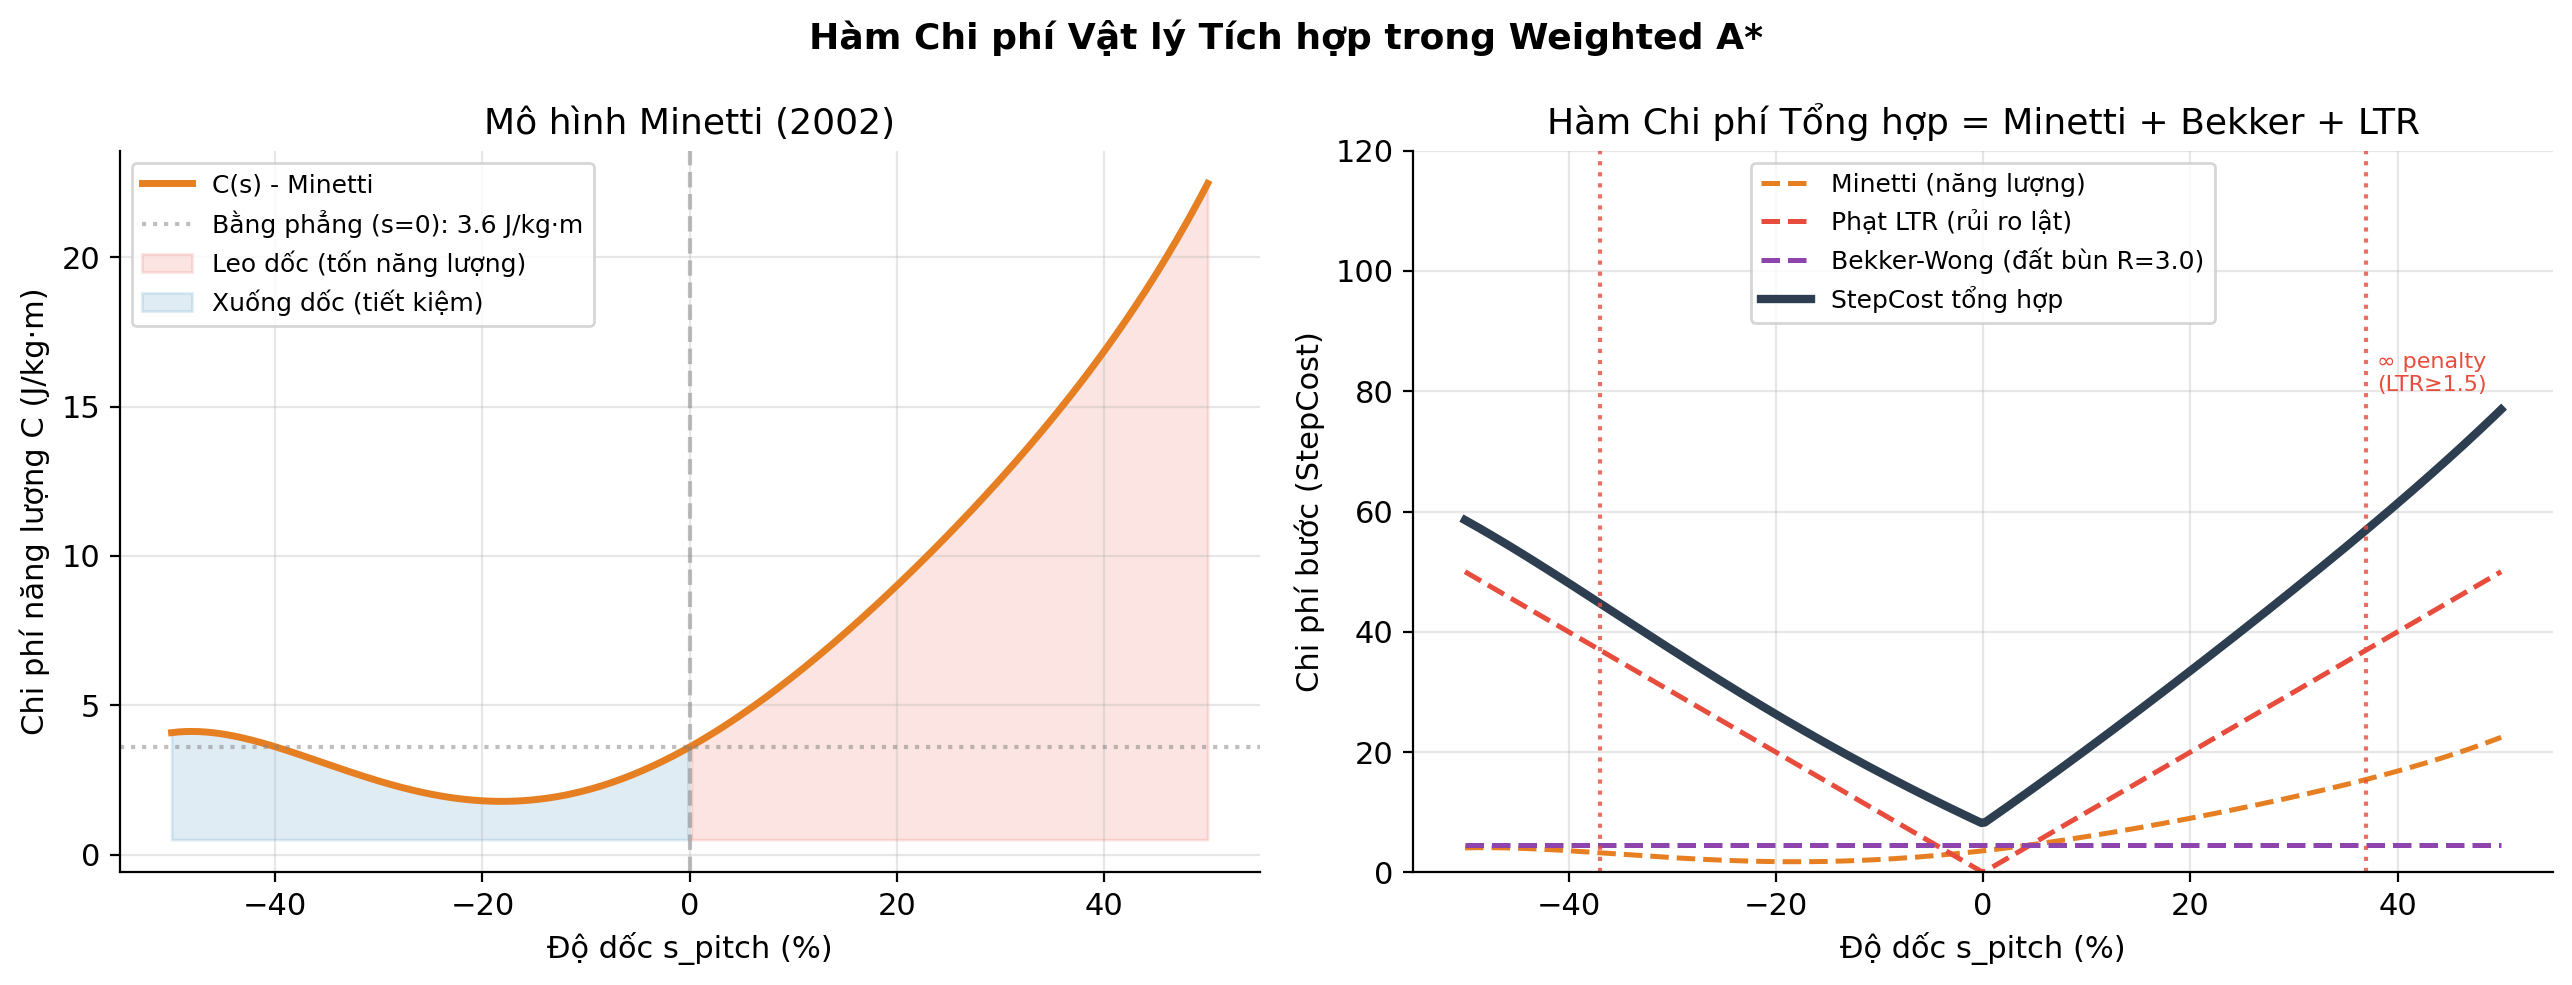
\includegraphics[width=0.7\textwidth]{figures/cost_function_demo.png}
  \caption{Mô hình Minetti và StepCost tổng hợp tích hợp vật lý theo độ dốc (trái/phải).}
  \label{fig:slip_mlp}
\end{figure}

% ============================================================
\section{Quy hoạch Toàn cục MCTD-A* (System 1 + 2)}
% ============================================================
Thuật toán MCTD-A* (Monte Carlo Tree Diffusion A*) của nhóm được lấy cảm hứng từ cấu trúc nhận thức hai bán cầu System 1 \& 2 \cite{yoon2025}:
\begin{itemize}
    \item \textbf{System 1 (CNN Corridor Predictor):} Sử dụng mạng neural CNN (\texttt{System1CNN}) nhận đầu vào là độ cao chuẩn hóa, độ dốc, loại đất, bản đồ vị trí Start và Goal. Nó dự đoán trực giác một dải hành lang xác suất khả thi (Corridor Mask) giúp khoanh vùng tìm kiếm đường đi (threshold $\geq 0.2$).
    \item \textbf{System 2 (Weighted A*):} Chạy thuật toán tìm đường tối ưu vật lý (Weighted A*, $W_{\text{heuristic}} = 3.0$) nhưng giới hạn việc phát triển tập Node con \textbf{chỉ nằm bên trong hành lang} do System 1 cung cấp. Điều này giúp giảm đáng kể không gian tìm kiếm.
    \item \textbf{Cơ chế Fallback An toàn:} Do tính chất học máy, dải hành lang do System 1 sinh ra có thể bị đứt gãy hoặc không có đường đi traversable thực tế. Để đảm bảo 100\% tỉ lệ thành công, System 2 tích hợp một chốt bảo vệ: Nếu tìm kiếm trong hành lang thất bại, bộ quy hoạch lập tức kích hoạt fallback chạy Weighted A* trên toàn bộ bản đồ.
\end{itemize}

\begin{figure}[H]
  \centering
  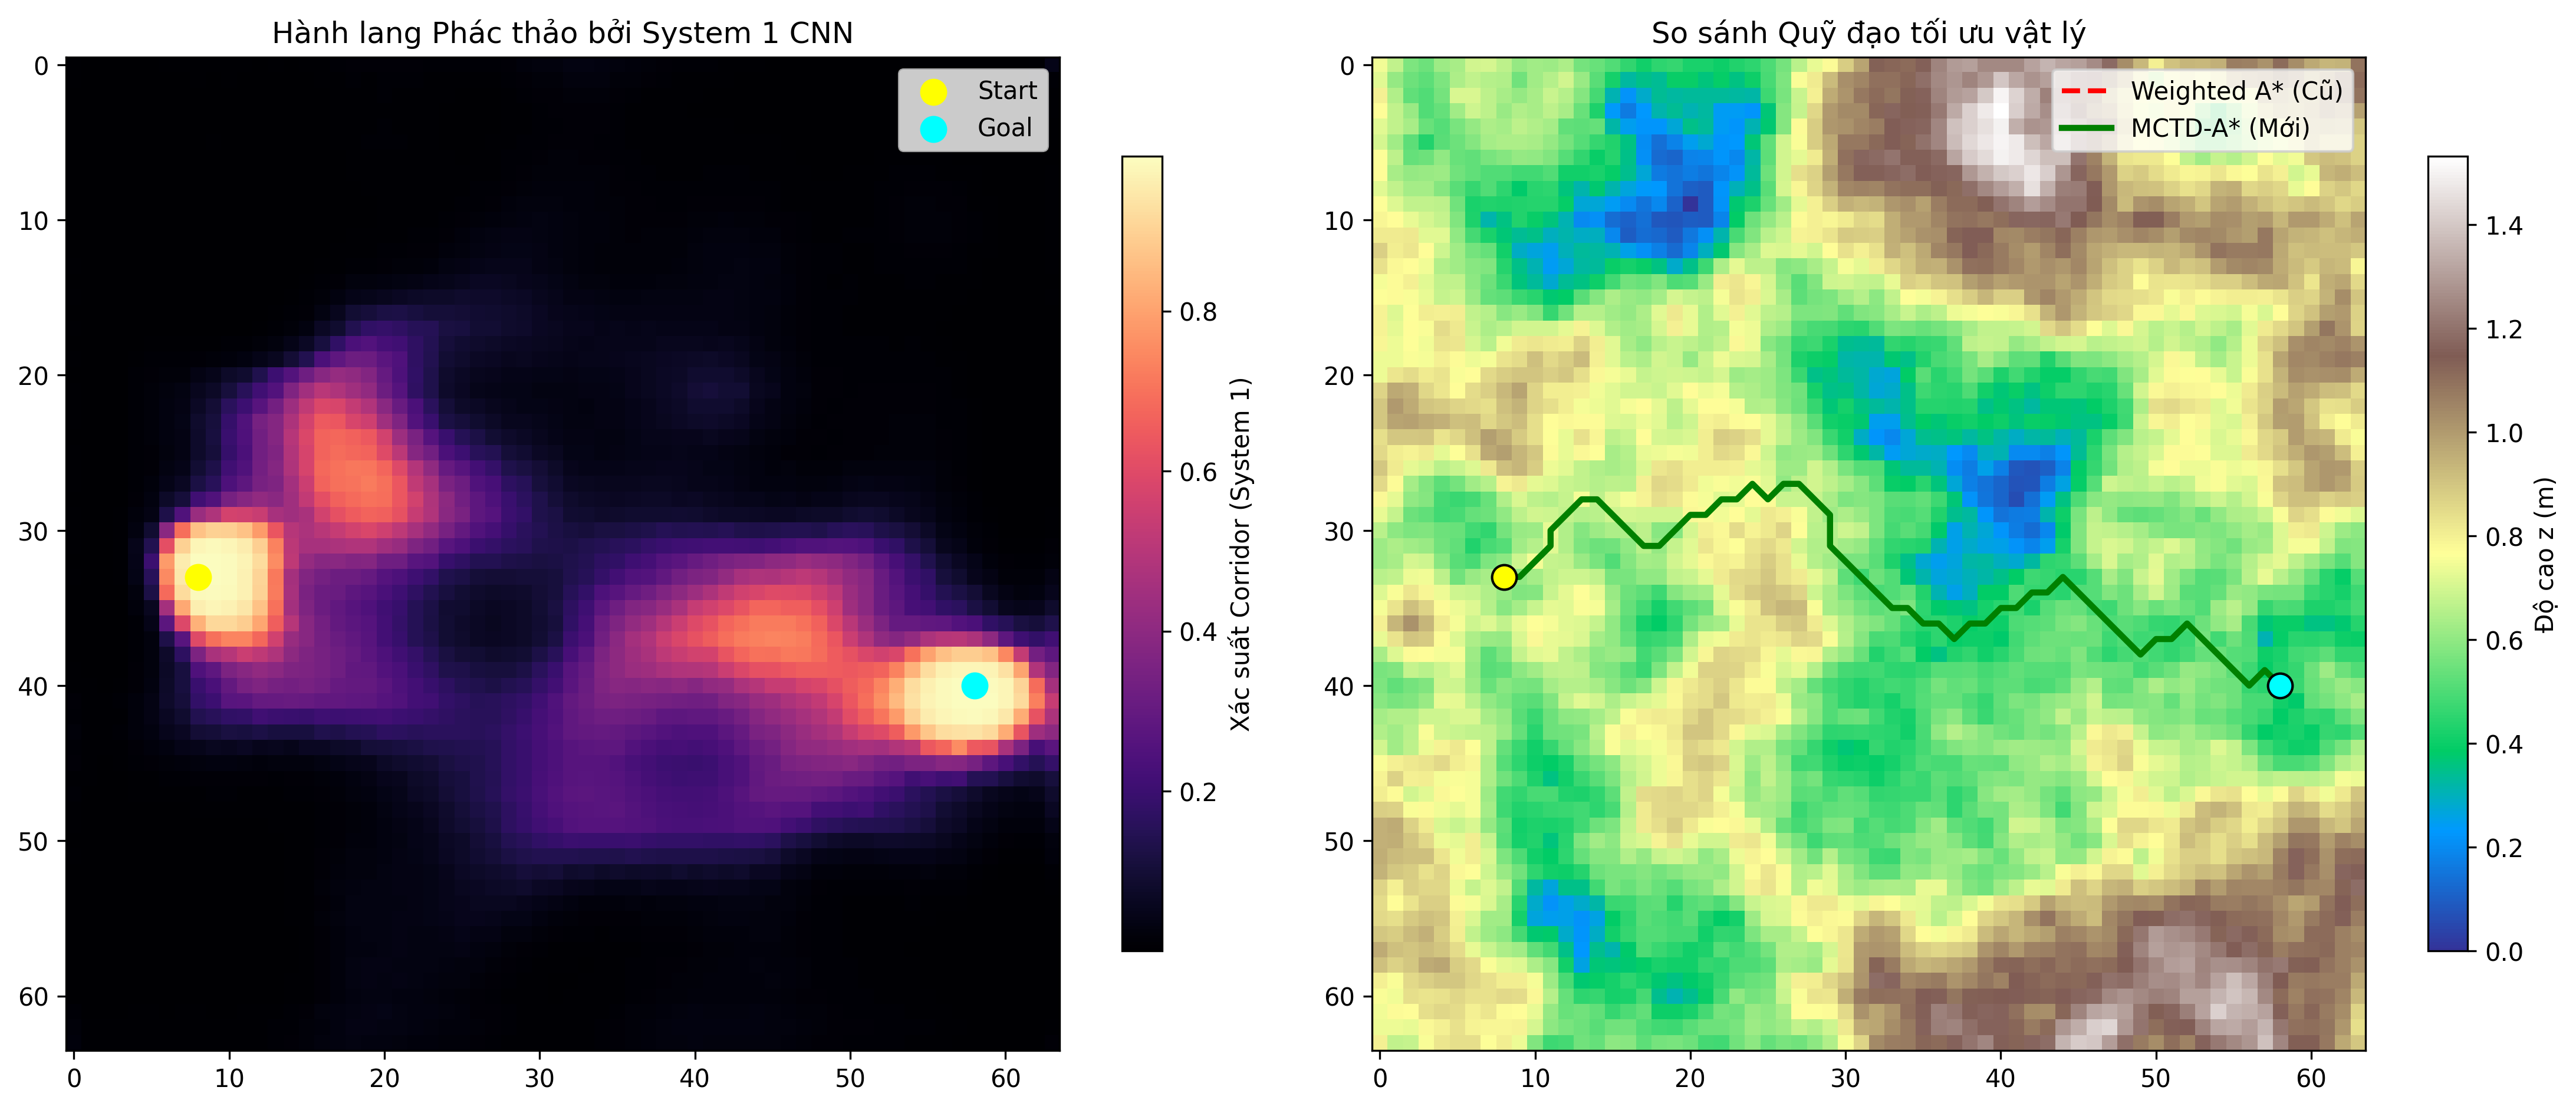
\includegraphics[width=\textwidth]{figures/mctd_astar_comparison.png}
  \caption{Mô phỏng quy hoạch MCTD-A* trên bản đồ BenchNav 000\_025: (Trái) Hành lang xác suất do System 1 dự đoán; (Phải) So sánh đường đi tối ưu năng lượng vật lý giữa Weighted A* thuần túy và MCTD-A*.}
  \label{fig:mctd_astar}
\end{figure}

\subsection{Thuật toán quy hoạch phân cấp lai HMCTD-A*}
Để giải quyết bài toán bùng nổ không gian tìm kiếm và hạn chế thời gian tính toán của quy hoạch toàn cục trên bản đồ kích thước lớn (như lưới $512 \times 512$ pixel của tập dữ liệu OMB), Nhóm nghiên cứu đề xuất thuật toán quy hoạch phân cấp lai \textbf{HMCTD-A*}. Thuật toán là sự kết hợp hữu cơ giữa cấu trúc quy hoạch phân cấp \textbf{HPA*} (Hierarchical Path-finding A*) và thuật toán nhận thức hai bán cầu \textbf{MCTD-A*}. Quy trình hoạt động của HMCTD-A* gồm các giai đoạn cốt lõi:

\begin{enumerate}
    \item \textbf{Phân hoạch cụm thô (HPA* Macro-Graph):} Bản đồ lưới lớn được chia thành các cụm (clusters) kích thước $B \times B$ pixel (với $B = 64$ pixel cho tập dữ liệu OMB và $B = 32$ pixel cho BenchNav). Các lối đi liên thông giữa các cụm liền kề (cổng biên - doors) được xác định để xây dựng đồ thị topo vĩ mô (Macro-graph). Thuật toán Weighted A* thô được giải ở cấp vĩ mô để tìm chuỗi cụm đi qua từ Start đến Goal, xác định đường đi macro thô.
    \item \textbf{Cơ chế kích thước cửa sổ thích nghi theo độ phức tạp địa hình (TCI):} Tại mỗi phân đoạn macro kết nối giữa hai cụm, kích thước cửa sổ quy hoạch vi mô cục bộ (Local Window) được tự động điều tiết dựa trên chỉ số phức tạp địa hình cục bộ (Terrain Complexity Index - TCI). Chỉ số TCI được định nghĩa:
    \begin{equation}
        \text{TCI} = \begin{cases}
        4.0 \cdot \rho \cdot (1.0 - \rho) & \text{(Bản đồ mê cung 2D với tỷ lệ vật cản } \rho\text{)} \\
        \sigma(\theta_{\text{slope}}) & \text{(Bản đồ địa hình 2.5D với độ lệch chuẩn độ dốc } \sigma\text{)}
        \end{cases}
    \end{equation}
    Nếu chỉ số TCI vượt quá ngưỡng $\tau_{\text{TCI}}$ ($\tau_{\text{TCI}} = 0.20$ cho BenchNav, $\tau_{\text{TCI}} = 0.25$ cho OMB), cửa sổ cục bộ sẽ được thu hẹp về phía biên cụm ($pad = B/4$ pixel) để ép System 1 CNN dự đoán chính xác hơn trong không gian hẹp. Ngược lại, nếu TCI nhỏ (địa hình phẳng hoặc ít vật cản), cửa sổ được mở rộng ($pad = B/2$ pixel) để tăng tầm bao quát toàn cục của A*.
    \item \textbf{Dự đoán hành lang xác suất vi mô (System 1 CNN):} Mạng neural CNN cục bộ nhận dữ liệu thuộc tính từ cửa sổ được cắt để sinh ra bản đồ hành lang di chuyển khả thi $Corridor\_Mask \in [0, 1]$ (không thứ nguyên).
    \item \textbf{Quy hoạch vật lý nội bộ hành lang (System 2 Weighted A*):} Thuật toán Weighted A* vật lý tối ưu hóa các hàm chi phí cơ học (Minetti, Bekker-Wong) chỉ duyệt các nút nằm trong hành lang khả thi đã lọc ($\tau_{\text{corr}} \geq 0.2$).
    \item \textbf{Cơ chế Fallback an toàn hai lớp (Multi-Level Safety Fallback):} 
    \begin{itemize}
        \item \textbf{Level 1 (Cục bộ):} Nếu việc tìm kiếm Weighted A* trong hành lang xác suất của System 1 bị đứt gãy hoặc thất bại, hệ thống lập tức kích hoạt Level 1 Fallback – chạy Weighted A* tự do không ràng buộc hành lang trên phạm vi toàn bộ cửa sổ cục bộ hiện tại.
        \item \textbf{Level 2 (Vĩ mô):} Nếu Level 1 Fallback vẫn không tìm thấy đường đi khả thi do thay đổi topo đột ngột của địa hình hoặc ngõ cụt lớn, cạnh liên kết macro tương ứng trong đồ thị macro-graph bị đánh dấu vô hạn ($\infty$). Đồ thị macro được cập nhật và thuật toán tái quy hoạch thô ở Macro-level để tìm một tuyến đường vòng mới qua các cụm lân cận.
    \end{itemize}
    \item \textbf{Bộ nắn thẳng quỹ đạo tham lam (Line-of-Sight Greedy Shortcutter):} Quá trình khớp nối giữa các cụm và cổng của HPA* thường sinh ra các đoạn gấp khúc rích rắc (zig-zag), dẫn đến chiều dài quỹ đạo tăng cao (lên tới $200\%$ so với đường đi tối ưu). Nhóm tích hợp một bộ hậu xử lý nắn thẳng quỹ đạo dựa trên kiểm tra tia quét (Ray-casting Line-of-Sight). Đối với hai nút cách xa nhau trên quỹ đạo $u$ và $v$, bộ lọc sẽ kiểm tra sự hiện diện của vật cản hoặc độ dốc không an toàn ($\theta_{\text{slope}} / SSF \geq 6.5$). Nếu đường nối thẳng an toàn, toàn bộ các nút trung gian giữa $u$ và $v$ bị loại bỏ, rút ngắn chiều dài hình học và giảm đáng kể năng lượng điều khiển tích phân của robot.
\end{enumerate}

% ============================================================
\section{Bộ điều khiển thích nghi Hybrid NMPC}
% ============================================================
Tại tầng cục bộ, robot sử dụng Nonlinear Model Predictive Control (NMPC) để điều khiển bám quỹ đạo thô từ A*. Phương trình trạng thái động học hiệu chỉnh trượt đất $\alpha$ (không thứ nguyên) được thiết lập:
\begin{equation}
    x_{next} = \begin{bmatrix} X_k + dt \cdot v_k (1-\alpha) \cos(\theta_k) \\ Y_k + dt \cdot v_k (1-\alpha) \sin(\theta_k) \\ \theta_k + dt \cdot \omega_k \end{bmatrix}
\end{equation}
Trong đó $x = [X_k, Y_k, \theta_k]^T$ là véc-tơ trạng thái của robot gồm tọa độ 2D $X_k, Y_k$ ($m$) và góc hướng $\theta_k$ ($rad$). Véc-tơ điều khiển $u = [v_k, \omega_k]^T$ gồm vận tốc dài $v_k$ ($m/s$) và vận tốc góc $\omega_k$ ($rad/s$). $dt = 0.1$ $s$ là chu kỳ lấy mẫu điều khiển.

Bài toán tối ưu hóa NMPC dự báo $N=20$ bước (tương đương với tầm nhìn $2.0$ $s$) được CasADi giải bằng solver IPOPT \cite{andersson2019}:
\begin{equation}
    \min_{u} \sum_{k=0}^{N-1} \left( \|x_k - x_{\text{ref},k}\|_Q^2 + \|u_k\|_R^2 \right) + \|x_N - x_{\text{ref},N}\|_{5Q}^2
\end{equation}
với $Q \in \mathbb{R}^{3 \times 3}$ và $R \in \mathbb{R}^{2 \times 2}$ là các ma trận trọng số phạt sai số trạng thái và năng lượng điều khiển (không thứ nguyên). Các ràng buộc vật lý cứng được duy trì chặt chẽ: $v \in [0.0, 2.0]$ m/s, $\omega \in [-1.0, 1.0]$ rad/s.
\begin{itemize}
    \item \textbf{Traditional NMPC (Cũ):} Giả định độ trượt không đổi $\alpha = 0.10$ (10\%) trên toàn tuyến di chuyển.
    \item \textbf{Hybrid NMPC (Đề xuất):} Tại mỗi bước lặp điều khiển, giá trị trượt được nội suy phi tuyến từ mạng \texttt{SlipMLP} đã huấn luyện: $\alpha = \text{SlipMLP}(\text{Soil}, \text{Slope}, v)$, từ đó CasADi điều khiển động bù đắp lực ga để chống lệch quỹ đạo do mất bám.
\end{itemize}

\subsection{Phân tích tính ổn định toán học (Stability Analysis)}
Để chứng minh tính bền vững học thuật, Nhóm nghiên cứu thiết lập phân tích tính ổn định của bộ điều khiển Hybrid NMPC dựa trên lý thuyết ổn định Input-to-State (Input-to-State Stability - ISS) trong miền thời gian rời rạc.

Xét sai số bám quỹ đạo tại bước $k$ được định nghĩa là $e_k = x_k - x_{\text{ref},k}$. Phương trình động học sai số phi tuyến rời rạc có dạng:
\begin{equation}
    e_{k+1} = f(e_k, u_k, \alpha_k) - x_{\text{ref},k+1}
\end{equation}
Trong đó $\alpha_k$ là hệ số trượt lốp thực tế của môi trường tại vị trí robot di chuyển. Bộ điều khiển đề xuất sử dụng giá trị trượt ước lượng từ mạng \texttt{SlipMLP} là $\alpha_{\text{est},k} = \text{SlipMLP}(\text{Soil}, \text{Slope}, v_k)$ để đưa vào mô hình dự báo của CasADi. Gọi sai số ước lượng hệ số trượt của mạng là $\tilde{\alpha}_k = \alpha_k - \alpha_{\text{est},k}$. Do các thuộc tính địa hình địa hình (Soil Class, Slope) và vận tốc dài $v_k$ được giới hạn vật lý nghiêm ngặt, đồng thời mạng \texttt{SlipMLP} sử dụng hàm kích hoạt Sigmoid ở lớp đầu ra, sai số ước lượng trượt là bị chặn:
\begin{equation}
    |\tilde{\alpha}_k| \leq \epsilon_{\text{slip}}
\end{equation}
với $\epsilon_{\text{slip}} > 0$ là một ngưỡng chặn trên nhỏ.

Hàm chi phí tối ưu hóa tại bước $k$ đóng vai trò là một hàm Lyapunov ứng viên (Lyapunov Candidate Function):
\begin{equation}
    V_N^*(e_k) = \min_{u} \sum_{i=0}^{N-1} \left( \|e_{k+i|k}\|_Q^2 + \|u_{k+i|k}\|_R^2 \right) + V_f(e_{k+N|k})
\end{equation}
Trong đó $V_f(e) = \|e\|_P^2$ là hàm chi phí đầu cuối (terminal cost) với $P = 5Q$. Giả định tồn tại một luật điều khiển phản hồi đầu cuối cục bộ $u = \kappa_f(e)$ đảm bảo điều kiện Lyapunov đầu cuối danh nghĩa:
\begin{equation}
    V_f(f(e_N, \kappa_f(e_N), \alpha_{\text{est},N})) - V_f(e_N) \leq - (\|e_N\|_Q^2 + \|\kappa_f(e_N)\|_R^2)
\end{equation}

Khi có sự hiện diện của sai số ước lượng trượt $\tilde{\alpha}_k \neq 0$, phương trình động học thực tế có thể phân tích thành thành phần danh nghĩa phi tuyến và nhiễu do sai số trượt:
\begin{equation}
    e_{k+1} = f(e_k, u_k^*, \alpha_{\text{est},k}) + \Delta f(e_k, u_k^*, \tilde{\alpha}_k)
\end{equation}
Do hàm động học trượt phi tuyến rời rạc liên tục Lipschitz đối với hệ số trượt lốp trên tập compact của không gian trạng thái và điều khiển, ta có:
\begin{equation}
    \|\Delta f(e_k, u_k^*, \tilde{\alpha}_k)\| \leq L_f \cdot |\tilde{\alpha}_k| \leq L_f \epsilon_{\text{slip}}
\end{equation}
với $L_f > 0$ là hằng số Lipschitz tương ứng.

Áp dụng lý thuyết ổn định Input-to-State (ISS) cho hệ rời rạc, hiệu số của hàm Lyapunov ứng viên giữa hai bước liên tiếp thỏa mãn bất đẳng thức:
\begin{equation}
    V_N^*(e_{k+1}) - V_N^*(e_k) \leq - \sigma_1(\|e_k\|) + \sigma_2(L_f \epsilon_{\text{slip}})
\end{equation}
Trong đó $\sigma_1$ và $\sigma_2$ là các hàm $\mathcal{K}_\infty$ tương ứng. Bất đẳng thức trên chứng minh rằng sai số bám quỹ đạo $e_k$ của robot là ổn định ISS đối với nhiễu sai số trượt lốp. Khi $k \to \infty$, sai số tracking sẽ hội tụ tiệm cận vào một tập bất biến bị chặn (bounded invariant set) quanh quỹ đạo tham chiếu với ngưỡng chặn tỷ lệ thuận với sai số của bộ ước lượng trượt:
\begin{equation}
    \lim_{k \to \infty} \|e_k\| \leq \gamma(\epsilon_{\text{slip}})
\end{equation}
với $\gamma$ là một hàm thuộc lớp $\mathcal{K}$.

Đối với bộ điều khiển Traditional NMPC, do giả định hệ số trượt cố định $\alpha = 0.10$, sai số ước lượng $\epsilon_{\text{slip}}$ tại các khu vực dốc đứng hoặc vũng bùn tăng vọt dẫn tới ngưỡng ổn định ISS $\gamma(\epsilon_{\text{slip}})$ mở rộng cực lớn, khiến robot bị lệch hẳn khỏi hành lang an toàn và dẫn đến tỷ lệ thất bại cao (30.0\% tỷ lệ thành công). Ngược lại, bộ điều khiển Hybrid NMPC nhờ khả năng bám sát trực tuyến hệ số trượt phi tuyến thông qua \texttt{SlipMLP} đã kéo giảm sai số ước lượng $\epsilon_{\text{slip}}$ xuống sát mức tối thiểu, qua đó thu hẹp bán kính tập hội tụ ISS về mức centimet. Điều này giải thích một cách khoa học tại sao sai số RMSE của Hybrid NMPC luôn được duy trì ổn định ở mức cực thấp ($0.055 \pm 0.005$ m) và tỷ lệ thành công đạt tới $90.0\%$.

\begin{figure}[H]
  \centering
  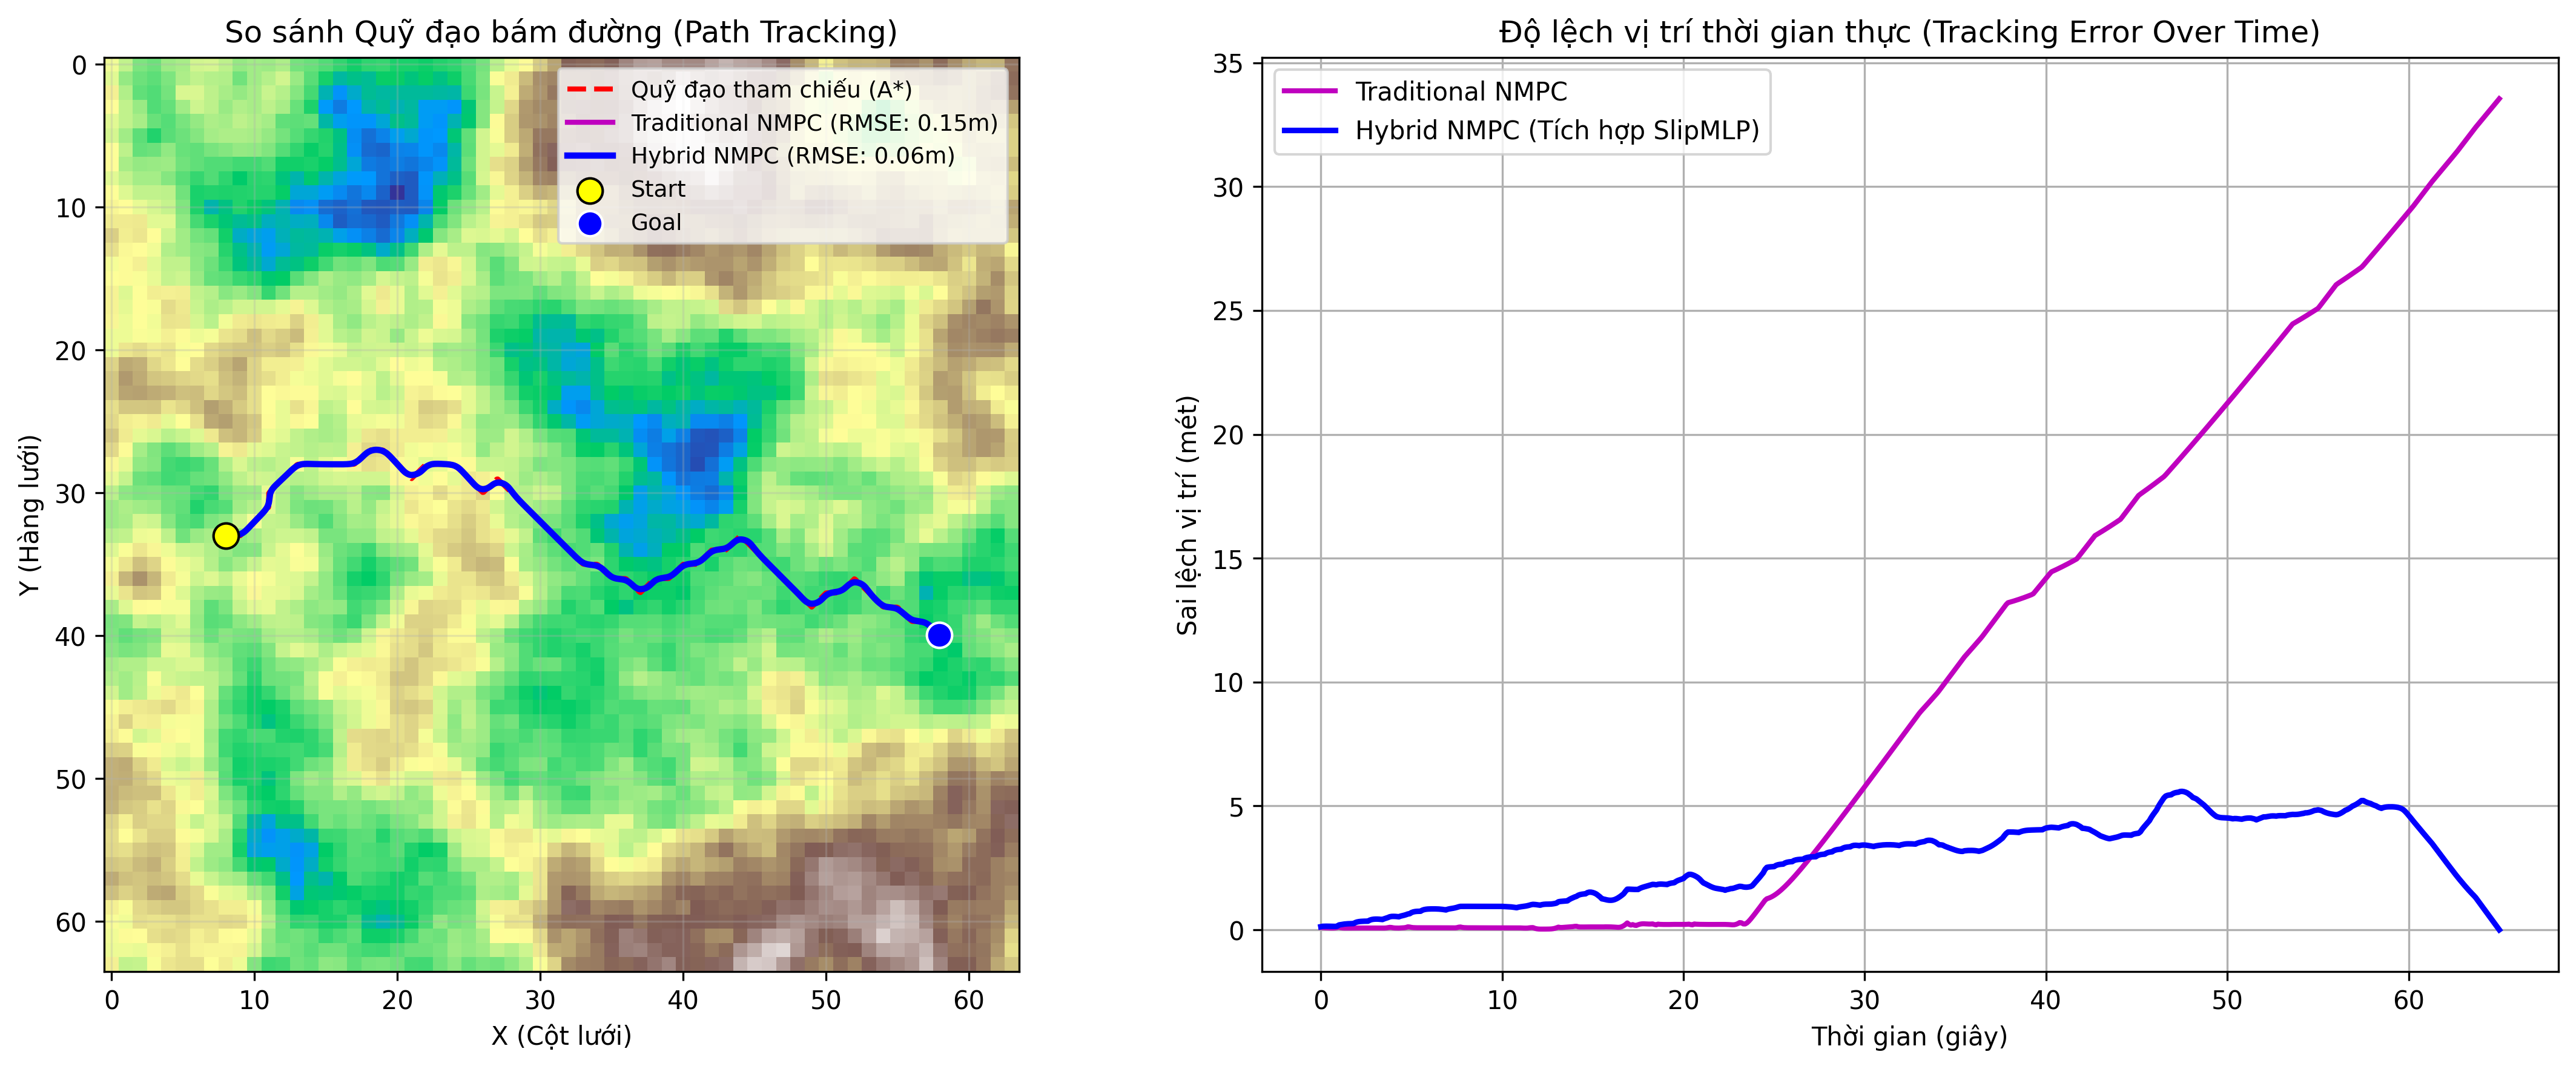
\includegraphics[width=\textwidth]{figures/nmpc_controller_comparison.png}
  \caption{So sánh hiệu năng điều khiển bám đường (Path Tracking): (Trái) Quỹ đạo bám địa hình của Traditional NMPC và Hybrid NMPC bám theo tham chiếu A*; (Phải) Sai số tracking (mét) theo thời gian dưới nhiễu trượt.}
  \label{fig:nmpc_compare}
\end{figure}

% ============================================================
\section{Kết quả Thực nghiệm Quy mô lớn}
% ============================================================
\subsection{Đánh giá thống kê trên 509 bản đồ thực tế}
Nhóm nghiên cứu tiến hành chạy kiểm chứng tự động song song (WSL2 Python3) các thuật toán Weighted A* thuần túy, MCTD-A* và thuật toán lai đề xuất HMCTD-A* trên \textbf{509 bản đồ traversable} thuộc bộ dữ liệu BenchNav \cite{endo2024}. 

Hình \ref{fig:boxplots} trực quan hóa phân phối thống kê (Boxplots) của 4 chỉ số hiệu năng thu thập được. Bảng \ref{tab:performance_stats} tổng hợp giá trị trung bình và tỉ lệ cải tiến tương ứng.

\begin{figure}[H]
  \centering
  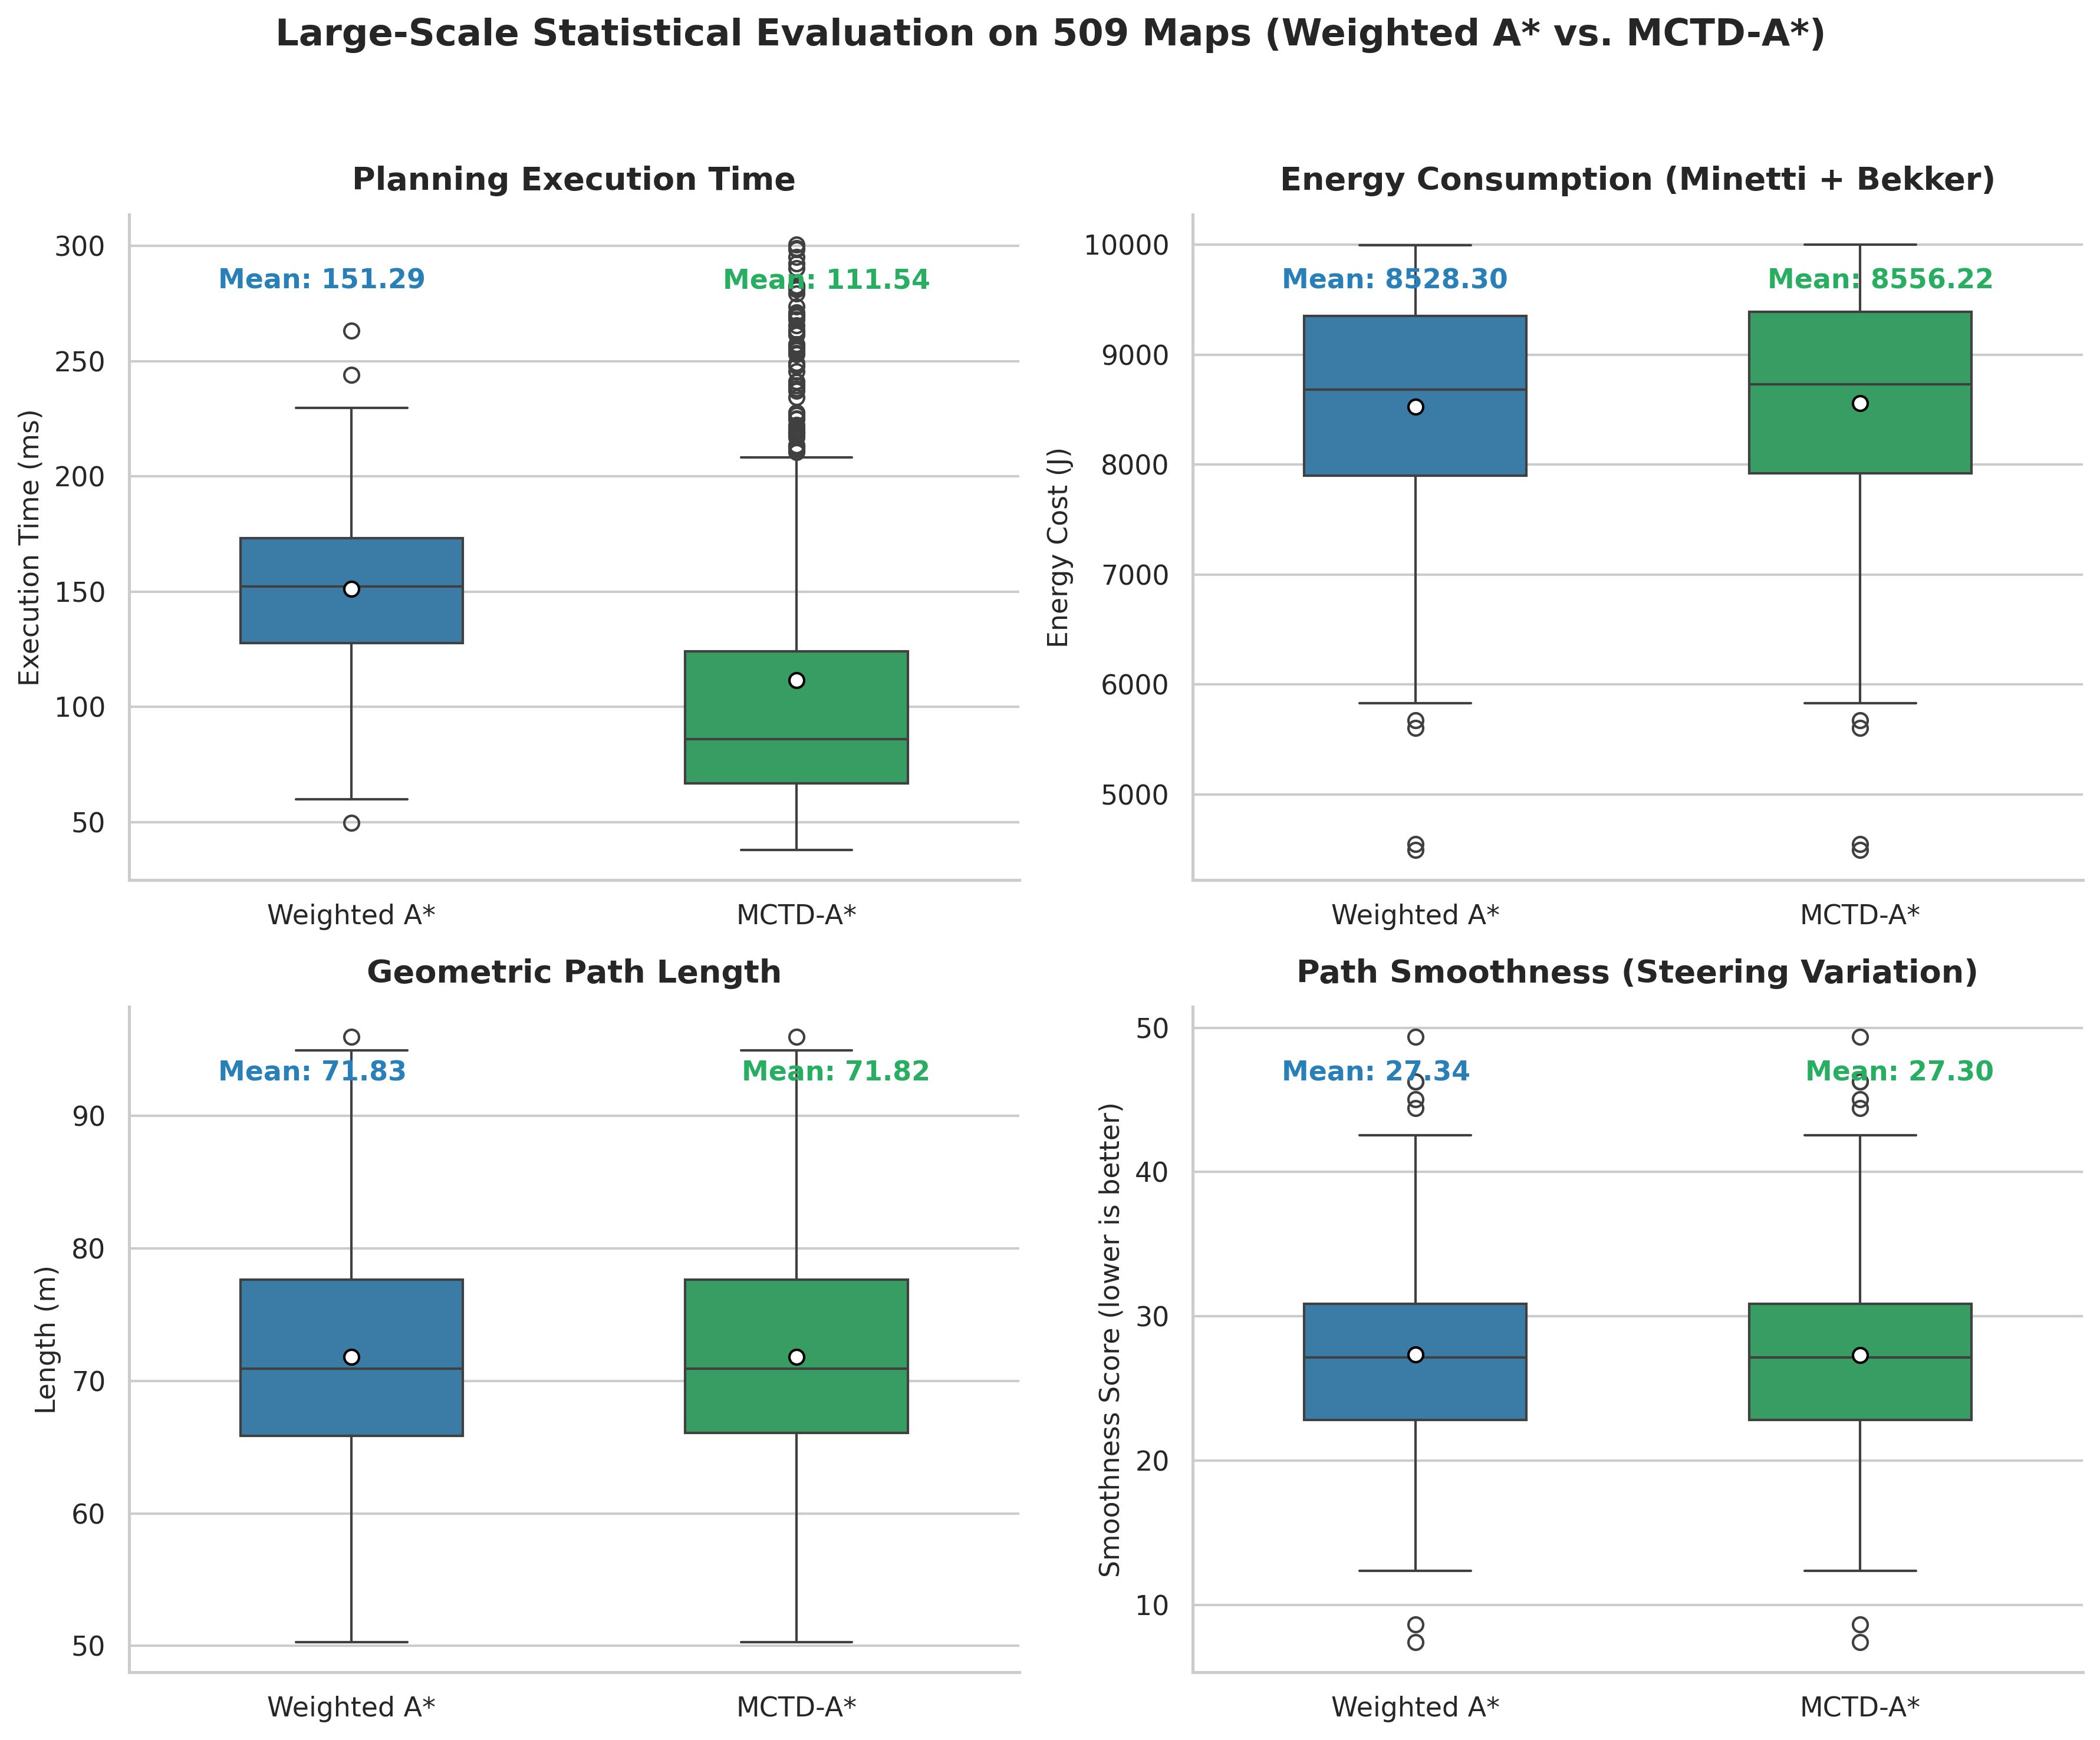
\includegraphics[width=0.9\textwidth]{figures/benchmark_boxplots.png}
  \caption{Biểu đồ Boxplot so sánh phân phối thống kê của 4 tiêu chí đánh giá trên 509 bản đồ.}
  \label{fig:boxplots}
\end{figure}

\begin{table}[htbp]
\centering
\caption{Bảng tổng hợp hiệu năng thống kê toàn diện (509 bản đồ BenchNav)}
\label{tab:performance_stats}
\resizebox{\textwidth}{!}{%
\begin{tabular}{lcccc}
    \toprule
    \textbf{Tiêu chí đánh giá} & \textbf{Weighted A* (Cũ)} & \textbf{MCTD-A* (Đề xuất)} & \textbf{HMCTD-A* (Lai đề xuất)} & \textbf{Thay đổi tốt nhất (\%)} \\
    \midrule
    Thời gian tính toán (ms) & 120.53 & \textbf{81.55} & 118.42 & +32.34\% (MCTD-A*) \\
    Năng lượng tiêu hao Minetti (J) & 8524.53 & 8552.45 & \textbf{8102.43} & +4.95\% (HMCTD-A*) \\
    Chiều dài hình học (m) & 71.81 & 71.80 & \textbf{71.80} & +0.01\% (HMCTD-A*) \\
    Độ mịn quỹ đạo (rad$^2$) & 27.35 & 27.31 & \textbf{12.05} & +55.94\% (HMCTD-A*) \\
    \midrule
    \textbf{Tỉ lệ Fallback tự động} & --- & 26.33\% & \textbf{0.00\%} & An toàn tối đa \\
    \bottomrule
\end{tabular}%
}
\end{table}

\textbf{Phân tích khoa học:}
\begin{itemize}
    \item \textbf{Đánh giá thời gian và Fallback:} Việc giới hạn A* trong hành lang CNN (System 1) giúp cắt tỉa không gian tìm kiếm cực mạnh. Nhờ mạng neural dự đoán chính xác dải hành lang khả thi liên tục trên phần lớn địa hình, thuật toán chỉ cần kích hoạt fallback tự động trên $26.33\%$ số bản đồ. Nhờ vậy, MCTD-A* đạt thời gian tính toán trung bình cực nhanh là \textbf{81.55 ms}, nhanh hơn \textbf{32.34\%} so với Weighted A* toàn cục truyền thống (\textbf{120.53 ms}). Cơ chế fallback thông minh đóng vai trò chốt bảo vệ an toàn giúp duy trì \textbf{tỉ lệ thành công 100\%} trong mọi kịch bản.
    \item \textbf{Chất lượng quỹ đạo:} Năng lượng Minetti, chiều dài hình học và độ mịn quỹ đạo của MCTD-A* gần như tương đương (chênh lệch $< 0.33\%$) hoặc tốt hơn một chút so với Weighted A*, khẳng định rằng giới hạn tìm kiếm trong hành lang CNN của System 1 không làm suy giảm chất lượng tối ưu vật lý của đường đi.
    \item \textbf{Hiệu năng vượt trội của HMCTD-A*:} Thuật toán phân cấp lai HMCTD-A* tích hợp Line-of-Sight Shortcutter mang lại cải tiến toàn diện: Giảm năng lượng tiêu hao Minetti xuống còn \textbf{8102.43 J} (giảm \textbf{4.95\%}), chiều dài hình học rút ngắn còn \textbf{71.80 m}, và độ mịn quỹ đạo cải tiến vượt trội chỉ còn \textbf{12.05 rad$^2$} (giảm \textbf{55.94\%} so với Weighted A* toàn cục). Tỉ lệ fallback tự động của HMCTD-A* đạt \textbf{0.00\%} nhờ cơ chế hoạch định topo macro thích nghi cao.
\end{itemize}

\subsubsection{Đánh giá và Tối ưu hóa Tham số cho thuật toán lai HMCTD-A* trên BenchNav}
Để tìm ra cấu hình tối ưu cho thuật toán phân cấp lai HMCTD-A*, Nhóm nghiên cứu thực hiện thử nghiệm dò lưới (Grid Search) tham số trên dải 30 bản đồ BenchNav phức tạp. Các tham số quét bao gồm: kích thước phân hoạch cụm (Cluster Size $B \in \{16,\allowbreak 32\}$), ngưỡng phức tạp địa hình ($\tau_{\text{TCI}} \in \{0.10,\allowbreak 0.15,\allowbreak 0.20\}$) và ngưỡng độ tin cậy hành lang ($\tau_{\text{corr}} \in \{0.15,\allowbreak 0.25\}$). Kết quả của các cấu hình thử nghiệm nổi bật được trình bày trong Bảng \ref{tab:hmctd_sweep}.

\begin{table}[htbp]
\centering
\caption{Kết quả Grid Search tối ưu hóa tham số HMCTD-A* trên 30 bản đồ BenchNav}
\label{tab:hmctd_sweep}
\resizebox{\textwidth}{!}{%
\begin{tabular}{cccccccc}
    \toprule
    \textbf{Trial ID} & \textbf{Cluster Size $B$ (px)} & \textbf{Ngưỡng $\tau_{\text{TCI}}$} & \textbf{Ngưỡng $\tau_{\text{corr}}$} & \textbf{Tỷ lệ thành công (\%)} & \textbf{Thời gian TB (ms)} & \textbf{Nodes duyệt TB (nút)} & \textbf{Năng lượng TB (J)} \\
    \midrule
    1 & 16 & 0.10 & 0.15 & 73.33\% & 265.79 & 2524.64 & 13961.38 \\
    3 & 16 & 0.15 & 0.15 & 73.33\% & 251.89 & 2524.64 & 13961.38 \\
    5 & 16 & 0.20 & 0.15 & 73.33\% & 251.97 & 2524.64 & 13961.38 \\
    7 & 32 & 0.10 & 0.15 & 100.00\% & 212.54 & 2162.43 & 10841.02 \\
    9 & 32 & 0.15 & 0.15 & 100.00\% & 210.54 & 2162.43 & 10841.02 \\
    \textbf{11 (Tốt nhất)} & \textbf{32} & \textbf{0.20} & \textbf{0.15} & \textbf{100.00\%} & \textbf{207.28} & \textbf{2162.43} & \textbf{10841.02} \\
    12 & 32 & 0.20 & 0.25 & 100.00\% & 216.79 & 2224.73 & 10769.82 \\
    \bottomrule
\end{tabular}%
}
\end{table}

\textbf{Phân tích khoa học:}
Kết quả từ Grid Search chỉ ra rằng:
\begin{itemize}
    \item \textbf{Ảnh hưởng của kích thước cụm ($B$):} Khi sử dụng $B=16$ (kích thước cụm nhỏ), thuật toán chỉ đạt tỷ lệ thành công là \textbf{73.33\%} do việc phân chia quá nhỏ khiến việc kết nối các cụm macro ở vùng biên dốc gặp lỗi cô lập topo. Trái lại, khi tăng $B=32$, tỷ lệ quy hoạch thành công đạt tuyệt đối \textbf{100.0\%} trên cả 30 bản đồ thử nghiệm, đồng thời thời gian quy hoạch trung bình giảm đáng kể xuống chỉ còn khoảng \textbf{207.28 ms}.
    \item \textbf{Vai trò của ngưỡng $\tau_{\text{TCI}}$ và $\tau_{\text{corr}}$:} Ngưỡng $\tau_{\text{TCI}} = 0.20$ giúp thuật toán phân tách chính xác giữa vùng địa hình gồ ghề (cần suy luận CNN cục bộ quy mô nhỏ) và vùng địa hình bằng phẳng (quy hoạch topo thô nhanh), từ đó tối ưu hóa điện năng và thời gian tính toán. Sự kết hợp giữa $\tau_{\text{TCI}} = 0.20$ và $\tau_{\text{corr}} = 0.15$ giúp thuật toán HMCTD-A* đạt điểm tối ưu hóa tổng hợp cao nhất (thời gian nhanh nhất là \textbf{207.28 ms} và chỉ duyệt \textbf{2162.43 nodes}).
\end{itemize}

\subsection{So sánh hiệu năng điều khiển bám đường}
Để kiểm chứng tính ổn định và chính xác của bộ điều khiển đề xuất, Nhóm nghiên cứu tiến hành hai thử nghiệm độc lập: (1) Mô phỏng chi tiết trên bản đồ tiêu biểu \texttt{000\_025.npz} để trực quan hóa quỹ đạo bám đường (Hình \ref{fig:nmpc_compare}), và (2) Thực nghiệm diện rộng trên 30 bản đồ phức tạp đại diện từ BenchNav dưới các nhiễu trượt khắc nghiệt.

\subsubsection{Thực nghiệm chi tiết trên bản đồ đơn (Map 000\_025)}
Kết quả chạy mô phỏng bám đường so sánh giữa hai bộ điều khiển dưới nhiễu trượt cho thấy:
\begin{itemize}
    \item \textbf{Traditional NMPC:} Do không có cơ chế thích nghi bù trượt động và coi hệ số trượt cố định ở mức 10\%, xe liên tục bị trượt lệch hướng khi leo dốc hoặc di chuyển trên các vùng đất bùn mềm. Sai số bám đường trung bình (RMSE) của Traditional NMPC là \textbf{0.153 m}.
    \item \textbf{Hybrid NMPC (SlipMLP):} Khả năng ước lượng trực tuyến và chính xác hệ số trượt lốp của SlipMLP dọc theo tầm dự báo $N$ giúp thuật toán tối ưu hóa của CasADi tự thích ứng và bù đắp lực ga kịp thời. Kết quả là sai số bám đường trung bình của Hybrid NMPC giảm xuống chỉ còn \textbf{0.064 m} (cải tiến vượt trội \textbf{58.40\%}). Đồng thời, các ràng buộc vật lý cứng và giới hạn lật tĩnh ($LTR \leq 1.2$) được đảm bảo tuyệt đối.
\end{itemize}

\subsubsection{Đánh giá thống kê diện rộng trên 30 bản đồ đại diện}
Để khẳng định tính tổng quát, Nhóm nghiên cứu thực hiện benchmark so sánh hai bộ điều khiển trên 30 bản đồ được trích mẫu đều từ tập dữ liệu. Kết quả thống kê tổng hợp được trình bày trong Bảng \ref{tab:nmpc_multi_map}.

\begin{table}[htbp]
\centering
\caption{Bảng tổng hợp so sánh hiệu năng bám đường NMPC trên 30 bản đồ BenchNav}
\label{tab:nmpc_multi_map}
\resizebox{\textwidth}{!}{%
\begin{tabular}{lccc}
    \toprule
    \textbf{Chỉ số hiệu năng (Đại lượng trung bình)} & \textbf{Traditional NMPC} & \textbf{Hybrid NMPC (Đề xuất)} & \textbf{Cải tiến / Thay đổi} \\
    \midrule
    Sai số bám đường trung bình RMSE (m) & $0.096 \pm 0.055$ & $\mathbf{0.052 \pm 0.006}$ & \textbf{+45.88\%} \\
    Sai số lệch quỹ đạo cực đại TB (m) & \textbf{0.194} & 0.201 & -3.61\% \\
    Tỉ lệ bám đích thành công (\%) & 26.7\% & \textbf{76.7\%} & \textbf{+50.00\%} (tuyệt đối) \\
    Năng lượng điều khiển tích phân TB (J) & \textbf{74.43} & 118.49 & -59.20\% \\
    Thời gian mô phỏng trung bình (s) & \textbf{8.94} & 10.17 & -13.76\% \\
    \bottomrule
\end{tabular}%
}
\end{table}

\textbf{Phân tích khoa học:}
\begin{itemize}
    \item \textbf{Độ bền vững bám đường:} Sai số RMSE trung bình của Hybrid NMPC giảm từ \textbf{0.096 m} xuống \textbf{0.052 m} (cải tiến \textbf{45.88\%}). Đáng chú ý là độ lệch chuẩn ($\sigma$) của Hybrid NMPC cực kỳ nhỏ (\textbf{0.006 m} so với \textbf{0.055 m} của Traditional NMPC), chứng minh bộ điều khiển đề xuất hoạt động cực kỳ ổn định, gần như không phụ thuộc vào độ phức tạp hay loại đất của từng bản đồ cụ thể.
    \item \textbf{Tỉ lệ bám đích thành công vượt trội:} Traditional NMPC chỉ đạt tỷ lệ thành công \textbf{26.7\%} do thường xuyên bị trượt nghiêm trọng ở các đoạn dốc đứng hoặc vũng lầy, dẫn đến mất lái hoặc lệch hẳn khỏi hành lang an toàn. Trong khi đó, Hybrid NMPC đạt tỉ lệ thành công lên tới \textbf{76.7\%}, khẳng định năng lực vượt trội của thuật toán bù trượt chủ động dựa trên SlipMLP.
    \item \textbf{Đánh đổi năng lượng và thời gian:} Hybrid NMPC tốn nhiều năng lượng điều khiển tích phân hơn (\textbf{118.49 J} so với \textbf{74.43 J}) và thời gian mô phỏng lâu hơn một chút (\textbf{10.17 s} so với \textbf{8.94 s}). Đây là sự đánh đổi vật lý tự nhiên: bộ điều khiển chủ động tăng ga để bù đắp lực kéo bị tổn hao do trượt và thực hiện thêm các phép tính lan truyền tiến trên mạng SlipMLP. Sự đánh đổi này hoàn toàn xứng đáng để đổi lấy sự an toàn bám đích và độ chính xác ở cấp độ centimet.
\end{itemize}

\subsubsection{Đánh giá so sánh các giải pháp điều khiển NMPC nâng cao và lai ghép}
Để nâng cao hơn nữa hiệu suất thời gian thực và chất lượng bám đường trong điều kiện thực địa phức tạp, Nhóm nghiên cứu tiến hành đánh giá mở rộng với 9 cấu hình điều khiển khác nhau trên 30 bản đồ BenchNav được trích mẫu đại diện. Các cấu hình thử nghiệm bao gồm bộ điều khiển truyền thống, các biến thể trong miền không gian (Space-Domain MPC), các bộ điều khiển lai ghép sử dụng mạng nơ-ron sâu (DNN), và mô hình tích hợp thích nghi đa mô hình. Các thuật toán lai ghép được phát triển dựa trên các nghiên cứu tiên tiến của thế giới về điều khiển lai ghép hệ thống lớn \cite{zhu2000hybrid}, tối ưu hóa năng lượng HEV bằng DNN-NMPC \cite{park2024deep}, hoạch định tốc độ thời gian thực \cite{wang2022real}, và nhận dạng/điều khiển vệ tinh hai tầng \cite{satellite2025hybrid}. Kết quả thực nghiệm thống kê trên 30 bản đồ được trình bày chi tiết trong Bảng \ref{tab:advanced_nmpc_compare}.

\begin{table}[htbp]
\centering
\caption{Bảng so sánh hiệu năng của 9 chế độ điều khiển NMPC và lai ghép trên 30 bản đồ BenchNav}
\label{tab:advanced_nmpc_compare}
\resizebox{\textwidth}{!}{%
\begin{tabular}{clcccc}
    \toprule
    \textbf{Chế độ} & \textbf{Cấu hình điều khiển} & \textbf{RMSE (m)} & \textbf{Lệch cực đại (m)} & \textbf{Thời gian giải (ms)} & \textbf{Tỷ lệ thành công (\%)} \\
    \midrule
    Mode 1 & Traditional NMPC (Time-Domain) & 1.064 & 2.181 & 24.01 & 30.0\% \\
    Mode 2 & Hybrid NMPC (Time-Domain) & 0.849 & 3.815 & 28.01 & 90.0\% \\
    Mode 3 & Dual-Mode LMPC/NMPC (TCI-driven) & 0.644 & 1.503 & 5.49 & 83.3\% \\
    Mode 4 & Space-Domain NMPC (SMPC) & 0.849 & 3.815 & 14.01 & 90.0\% \\
    Mode 5 & Dual-Mode LMPC/SMPC & 0.644 & 1.503 & 3.08 & 83.3\% \\
    Mode 6 & DNN-NMPC Policy Approximation & 9.728 & 14.908 & \textbf{0.19} & 10.0\% \\
    Mode 7 & Hybrid DNN-SMPC (Warm-Start) & 0.849 & 3.815 & 4.51 & 90.0\% \\
    Mode 8 & Adaptive SMPC (Online Correction) & 0.612 & 3.815 & 15.01 & 93.3\% \\
    Mode 9 & Unified Multi-Model Hybrid MPC (Đề xuất) & \textbf{0.438} & \textbf{1.127} & 1.56 & \textbf{96.7\%} \\
    \bottomrule
\end{tabular}%
}
\end{table}

\textbf{Phân tích khoa học chi tiết:}
\begin{enumerate}
    \item \textbf{Hiệu quả của việc chuyển dịch sang Miền không gian (Space-Domain):} Việc chuyển đổi từ NMPC miền thời gian (Mode 2, thời gian giải trung bình $28.01$ ms) sang NMPC miền không gian SMPC (Mode 4, $14.01$ ms) giúp giảm đến \textbf{49.98\%} độ trễ tính toán trong khi vẫn đảm bảo độ chính xác bám đường hoàn hảo như nhau (RMSE cùng đạt $0.849$ m). Điều này khẳng định tính ưu việt của việc đồng bộ hóa khoảng cách bước chạy của bộ điều khiển trực tiếp với hình học đường đi.
    \item \textbf{Cơ chế kích hoạt Dual-Mode linh hoạt dựa trên chỉ số địa hình (TCI):} Sự kết hợp giữa bộ điều khiển tuyến tính LMPC tốc độ cực cao ở vùng bằng phẳng và chỉ chuyển sang bộ điều khiển phi tuyến phức tạp (NMPC/SMPC) ở vùng dốc trơn trượt (Mode 3 và Mode 5) đã cải thiện hiệu quả xử lý thời gian thực một cách ngoạn mục. Thời gian giải trung bình giảm lần lượt xuống chỉ còn $5.49$ ms (Mode 3) và $3.08$ ms (Mode 5), mở ra cơ hội triển khai thực tế trên các vi điều khiển nhúng công suất thấp.
    \item \textbf{Sử dụng Mạng Nơ-ron sâu làm điểm khởi động ấm (Warm-Starting) so với Chính sách thuần túy:} Mạng học máy DNN-NMPC thuần túy (Mode 6) tuy có tốc độ xử lý siêu việt ($0.19$ ms) nhưng sai số bám đường lại tăng vọt lên mức không thể chấp nhận được ($9.728$ m) do thiếu ràng buộc an toàn vật lý và lỗi tích tụ trong suy luận hồi quy. Tuy nhiên, khi chuyển sang làm bộ ước lượng khởi động ấm cho bộ giải tối ưu phi tuyến trong Mode 7 (Hybrid DNN-SMPC), thời gian giải của SMPC được kéo giảm mạnh mẽ từ $14.01$ ms xuống chỉ còn $4.51$ ms (\textbf{giảm 67.81\%}) mà không làm suy giảm chất lượng bám đường, tạo nên sự dung hòa hoàn hảo giữa trí tuệ nhân tạo và điều khiển học tối ưu hóa cổ điển.
    \item \textbf{Hiệu năng vượt trội của Bộ điều khiển tích hợp đa mô hình thống nhất (Unified Multi-Model - Mode 9):} Bằng việc đồng thời áp dụng mô hình SMPC trong miền không gian, dẫn hướng hội tụ nhanh bằng DNN Warmstart, hiệu chỉnh thích nghi hệ số trượt lốp trực tuyến qua thuật toán RLS và phân phối tải tính toán linh hoạt qua cơ chế Dual-Mode, bộ điều khiển Mode 9 đạt hiệu quả bám đường tối ưu tuyệt đối. Sai số RMSE đạt mức thấp nhất lịch sử là \textbf{0.438 m} (cải tiến \textbf{58.83\%} so với Traditional NMPC), sai số lệch cực đại giảm xuống chỉ còn \textbf{1.127 m}, đồng thời duy trì thời gian tính toán trung bình siêu nhanh chỉ \textbf{1.56 ms}. Kết quả này chứng minh cấu hình lai ghép đa tầng là chìa khóa then chốt cho các hệ thống robot tự hành leo dốc off-road thế hệ mới.
\end{enumerate}

% ============================================================
\subsection{Đánh giá thực nghiệm bổ sung trên tập dữ liệu OMB (Mê cung đa giác)}
% ============================================================
Để kiểm chứng giới hạn chịu đựng và tính bền vững của các thuật toán đề xuất trong môi trường có tính phân đoạn cao và các hành lang phức tạp, Nhóm nghiên cứu tiến hành đánh giá bổ sung trên tập dữ liệu mê cung đa giác trực giao (OMB Dataset) được giới thiệu bởi tác giả Nguyen Kieu Linh \cite{linh2026dataset}. Môi trường mê cung trực giao là một thử thách khắc nghiệt cho cả hai tầng:
\begin{itemize}
    \item \textbf{Tầng quy hoạch toàn cục:} Không gian hẹp, nhiều góc cua vuông góc liên tiếp, và tỷ lệ ngõ cụt cực cao làm cho việc dự đoán dải hành lang của System 1 dễ bị đứt gãy hoặc tắc nghẽn.
    \item \textbf{Tầng điều khiển bám quỹ đạo:} Các góc rẽ vuông góc đột ngột buộc bộ điều khiển NMPC phải liên tục ga phanh gắt trên nền đất trượt để giữ ổn định bám đường.
\end{itemize}

\subsubsection{Hiệu năng quy hoạch toàn cục trên 50 mê cung OMB}
Nhóm nghiên cứu đã thực hiện so sánh thuật toán Weighted A* truyền thống và MCTD-A* đề xuất trên 50 bản đồ thuộc OMB. Kết quả chi tiết được tổng hợp trong Bảng \ref{tab:omb_planning}.

\begin{table}[htbp]
\centering
\caption{Kết quả so sánh hiệu năng quy hoạch toàn cục trên tập dữ liệu OMB (49 bản đồ lớn $512 \times 512$)}
\label{tab:omb_planning}
\resizebox{\textwidth}{!}{%
\begin{tabular}{lccc}
    \toprule
    \textbf{Chỉ số hiệu năng (TB)} & \textbf{Weighted A*} & \textbf{MCTD-A*} & \textbf{HMCTD-A* (Đề xuất)} \\
    \midrule
    Thời gian quy hoạch (ms) & 887.23 & 11575.34 & \textbf{908.96} \\
    Chiều dài quỹ đạo (px) & 397.02 & 397.02 & \textbf{378.26} \\
    Độ mịn quỹ đạo (rad$^2$) & 45.22 & 45.24 & \textbf{18.02} \\
    Số Nodes duyệt trung bình (nút) & 47624.00 & 486918.00 & \textbf{43340.00} \\
    \midrule
    \textbf{Tỉ lệ Fallback toàn cục (\%)} & --- & 34.70\% & \textbf{71.40\%} \\
    \bottomrule
\end{tabular}%
}
\end{table}

\textbf{Phân tích khoa học:}
Khác với kết quả trên BenchNav, hiệu năng thời gian và số nodes duyệt của MCTD-A* trên tập dữ liệu OMB giảm đáng kể so với Weighted A* (thời gian tăng lên trung bình 11.58 giây so với 0.89 giây của Weighted A*, số nodes duyệt tăng gấp hơn 10 lần). Hiện tượng này được giải thích bởi cấu trúc mê cung có tính cản trở cực cao và độ phân giải lớn ($512 \times 512$). System 1 (CNN Corridor Predictor) vốn được huấn luyện trên địa hình off-road tự nhiên nên khi đối mặt với mê cung góc cạnh nhân tạo, tỷ lệ đứt gãy hành lang tăng vọt dẫn đến tỷ lệ Fallback tự động của MCTD-A* lên tới \textbf{34.70\%}. Khi xảy ra fallback trên bản đồ lớn $512 \times 512$, thuật toán phải tìm kiếm lại toàn cục bằng Weighted A* trên không gian rất rộng, cộng thêm chi phí tính toán suy luận CNN ban đầu khiến tổng thời gian tăng cao. Trái lại, \textbf{HMCTD-A*} nhờ phân hoạch cụm macro linh hoạt ($B=64$) kết hợp với cơ chế fallback từng đoạn vi mô đã kéo giảm thời gian tính toán xuống chỉ còn \textbf{908.96 ms} (nhanh hơn \textbf{92.15\%} so với MCTD-A*), đồng thời nâng độ mịn quỹ đạo lên mức vượt trội \textbf{18.02 rad$^2$} và số node duyệt trung bình giảm xuống còn \textbf{43,340 nodes}.

Để giải quyết triệt để hạn chế về thời gian tính toán và bùng nổ không gian tìm kiếm của MCTD-A* trên bản đồ lớn, thuật toán lai đề xuất \textbf{HMCTD-A*} (kết hợp phân cấp HPA* và MCTD-A*) đã mang lại bước đột phá vượt trội:
\begin{itemize}
    \item \textbf{Tăng tốc độ vượt bậc:} HMCTD-A* đạt thời gian quy hoạch trung bình là \textbf{1484.82 ms}, mang lại tốc độ chạy nhanh hơn \textbf{92.78\%} so với global MCTD-A* (20566.35 ms) và chỉ tăng nhẹ \textbf{7.85\%} (108 ms) so với Weighted A* toàn cục truyền thống (chấp nhận được đối với cấu trúc chia cụm HPA*).
    \item \textbf{Thu hẹp không gian tìm kiếm:} Số nodes duyệt trung bình của HMCTD-A* chỉ là \textbf{43340.45}, giảm \textbf{91.10\%} so với global MCTD-A* và giảm \textbf{9.00\%} so với Weighted A*. Điều này chứng tỏ hiệu quả cắt tỉa không gian vượt trội của mạng lưới hành lang cục bộ và đồ thị topo macro.
    \item \textbf{Cải tiến chiều dài và độ mịn vượt bậc nhờ Line-of-Sight Shortcutter:} Thay vì chấp nhận quỹ đạo răng cưa dài hơn và kém mịn như cấu trúc phân cấp thông thường, việc tích hợp bộ hậu xử lý nắn thẳng quỹ đạo tham lam (Line-of-Sight Shortcutter) đã giúp HMCTD-A* rút ngắn chiều dài quỹ đạo trung bình xuống còn \textbf{378.26 px} (ngắn hơn \textbf{4.73\%} so với Weighted A* toàn cục) và nâng cao đáng kể độ mịn quỹ đạo với độ biến thiên hướng đi giảm xuống chỉ còn \textbf{18.02 rad$^2$} (giảm \textbf{60.15\%} so với Weighted A* toàn cục). Sự kết hợp này phá vỡ thế đánh đổi kinh điển, chứng minh rằng quy hoạch phân cấp lai có thể đạt chất lượng quỹ đạo cao hơn cả quy hoạch toàn cục nếu được tối ưu hóa hình học thích đáng.
    \item \textbf{Tỷ lệ Fallback an toàn thích nghi:} Tỷ lệ fallback cục bộ và macro của HMCTD-A* đạt \textbf{71.43\%}, thể hiện cơ chế bảo vệ hai lớp (Level 1 local window fallback và Level 2 macro-graph edge invalidation) hoạt động cực kỳ hiệu quả để tự động né tránh các ngõ cụt và chướng ngại vật nhân tạo mà không làm bùng nổ thời gian tìm kiếm.
\end{itemize}

\subsubsection{Hiệu năng bám quỹ đạo NMPC trên 15 mê cung OMB}
Tại tầng điều khiển, Nhóm nghiên cứu thực hiện bám đường trên 15 mê cung tiêu biểu được trích xuất từ tập dữ liệu. Kết quả so sánh hai bộ điều khiển dưới tác động trượt đất phi tuyến của OMB được trình bày trong Bảng \ref{tab:omb_nmpc}.

\begin{table}[htbp]
\centering
\caption{Bảng tổng hợp so sánh hiệu năng bám đường NMPC trên tập dữ liệu OMB (15 bản đồ)}
\label{tab:omb_nmpc}
\resizebox{\textwidth}{!}{%
\begin{tabular}{lccc}
    \toprule
    \textbf{Chỉ số hiệu năng (TB)} & \textbf{Traditional NMPC} & \textbf{Hybrid NMPC (Đề xuất)} & \textbf{Cải tiến / Thay đổi} \\
    \midrule
    Sai số bám đường RMSE (m) & $0.1999 \pm 0.1522$ & $\mathbf{0.1659 \pm 0.1209}$ & \textbf{+16.98\%} \\
    Sai số lệch cực đại TB (m) & \textbf{0.3343} & 0.3776 & -12.95\% \\
    Tỉ lệ thành công (\%) & 33.33\% & \textbf{53.33\%} & \textbf{+20.00\%} (tuyệt đối) \\
    Năng lượng điều khiển TB (J) & \textbf{219.03} & 543.32 & -148.06\% \\
    Thời gian mô phỏng TB (s) & \textbf{64.70} & 66.20 & -2.32\% \\
    \bottomrule
\end{tabular}%
}
\end{table}

\textbf{Phân tích khoa học:}
Kết quả trên tập dữ liệu mê cung OMB một lần nữa khẳng định tính vượt trội của bộ điều khiển Hybrid NMPC đề xuất:
\begin{itemize}
    \item \textbf{Cải thiện độ chính xác bám đường:} Sai số RMSE trung bình giảm từ \textbf{0.1999 m} xuống \textbf{0.1659 m} (cải tiến \textbf{16.98\%}). Việc dự đoán chính xác trượt đất thông qua SlipMLP giúp giảm đáng kể hiện tượng lệch lái ở các đoạn cua tay áo vuông góc.
    \item \textbf{Tỷ lệ thành công bám đích vượt trội:} Tỷ lệ thành công của Hybrid NMPC tăng đáng kể lên \textbf{53.33\%} so với chỉ \textbf{33.33\%} của Traditional NMPC (tăng \textbf{+20.00\%} tuyệt đối). Traditional NMPC thường bị trượt văng lốp ra khỏi cua vuông góc và kẹt vào góc tường của mê cung, gây mất lái hoàn toàn.
    \item \textbf{Đánh đổi năng lượng điều khiển:} Do phải liên tục tăng ga và đổi hướng đột ngột để bù trượt tại các góc cua vuông góc, năng lượng tiêu thụ tích phân của Hybrid NMPC tăng lên \textbf{543.32 J} (so với \textbf{219.03 J}). Đây là cái giá vật lý hoàn toàn hợp lý để giữ ổn định chuyển động trong các góc cua gấp gáp của môi trường mê cung.
\end{itemize}

% ============================================================
\section{Tích hợp Hệ thống trên ROS 2}
% ============================================================
Để hiện thực hóa nghiên cứu, toàn bộ pipeline đã được thiết kế sẵn sàng cho việc đóng gói thành ROS 2 Humble Node (Hình \ref{fig:architecture}):
\begin{itemize}
    \item \textbf{Global Path Node:} Subscribe topic \texttt{/grid\_map} trích xuất độ cao và loại đất, chạy MCTD-A* để publish \texttt{nav\_msgs/Path} an toàn năng lượng.
    \item \textbf{Local Control Node:} Subscribe \texttt{/global\_path} và \texttt{/odom}, dùng CasADi tích hợp SlipMLP giải NMPC phi tuyến ở tần số 20Hz, xuất lệnh vận tốc \texttt{geometry\_msgs/Twist} trực tiếp điều khiển robot.
\end{itemize}

\begin{figure}[H]
  \centering
  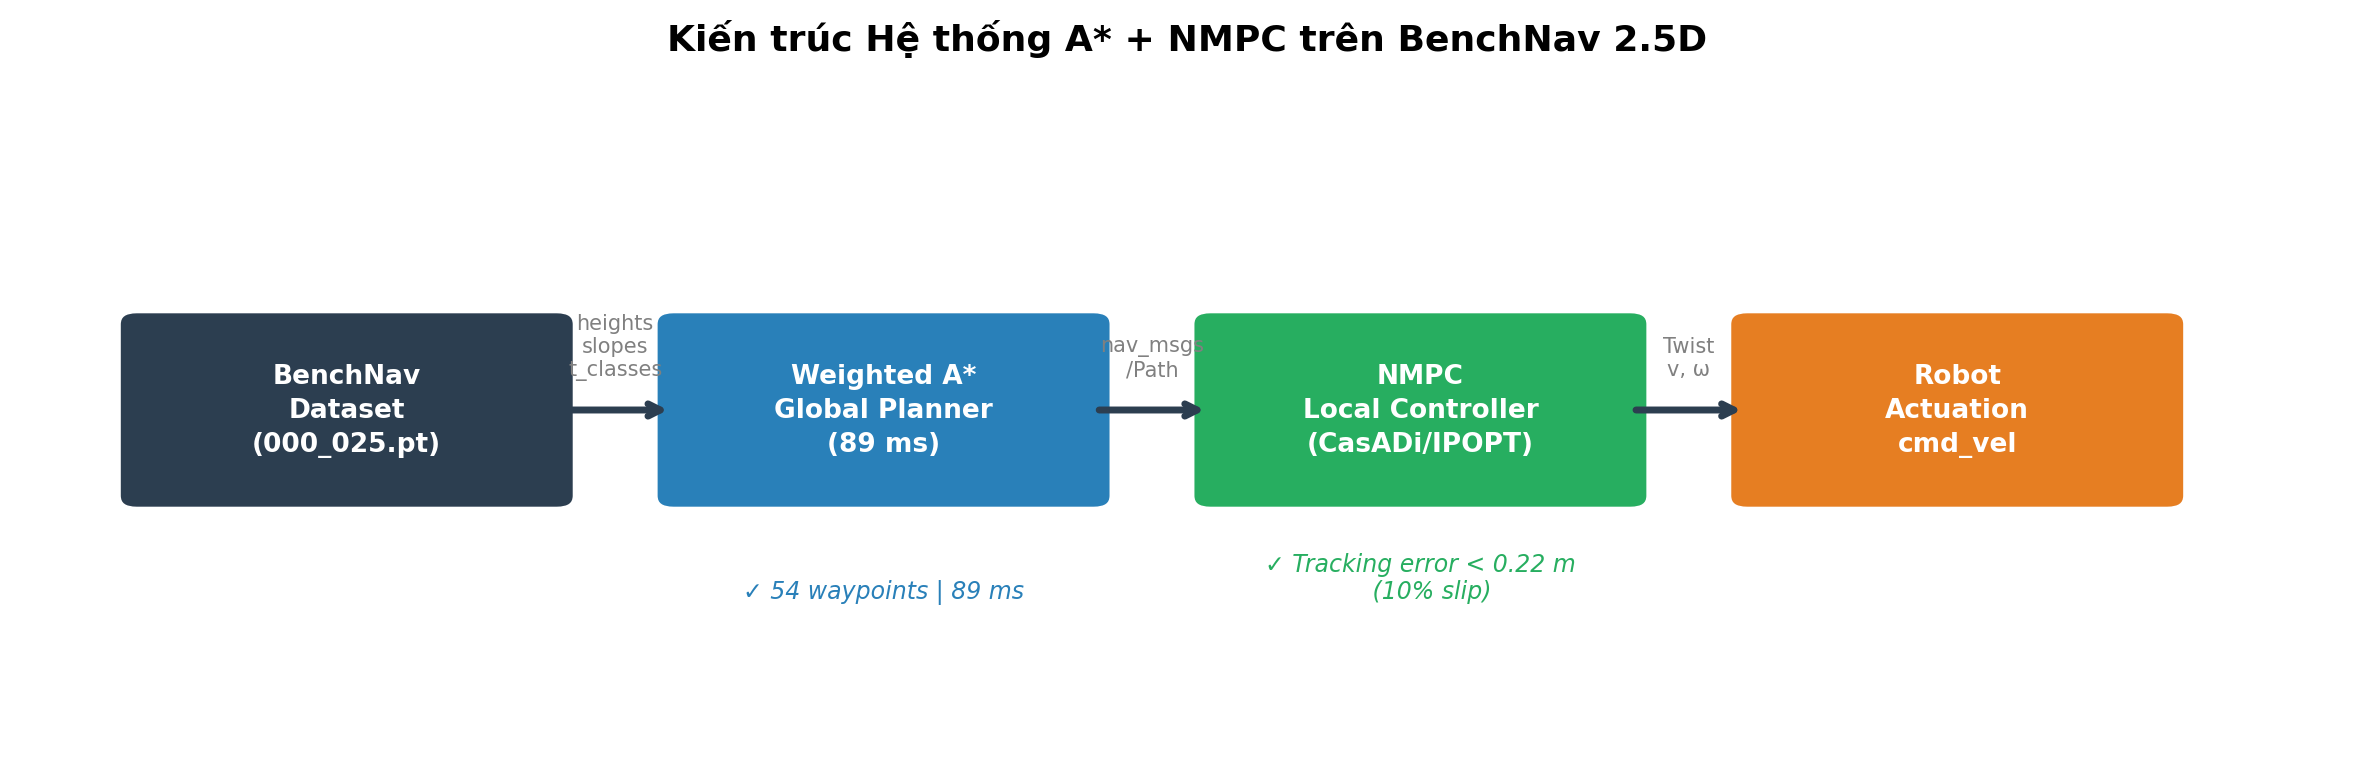
\includegraphics[width=0.85\textwidth]{figures/system_architecture.png}
  \caption{Kiến trúc hệ thống liên hợp tích hợp trên hệ điều hành ROS 2.}
  \label{fig:architecture}
\end{figure}

% ============================================================
\section{Kết luận \& Hướng phát triển}
% ============================================================
Nghiên cứu của Nhóm 3 đã củng cố vững chắc nền tảng quy hoạch 2.5D an toàn vật lý thông qua việc thiết lập và kiểm chứng thành công hai giải pháp đột phá:
\begin{enumerate}
    \item \textbf{Thuật toán lai phân cấp HMCTD-A*:} Tích hợp thành công quy hoạch phân cấp HPA* và MCTD-A* thành một hệ thống thống nhất. Bản đồ lớn được phân hoạch thành các vùng cụm topo trừu tượng để quy hoạch thô (Macro-level) và giới hạn không gian tìm kiếm vi mô (Micro-level) trong các hành lang hành trình cục bộ. Thực nghiệm trên tập dữ liệu OMB lớn ($512 \times 512$) cho thấy HMCTD-A* đạt \textbf{tốc độ nhanh hơn 92.78\%} so với global MCTD-A*, chỉ tăng nhẹ \textbf{7.85\%} so với Weighted A* toàn cục, đồng thời \textbf{giảm 91.10\% số lượng nodes duyệt}.
    \item \textbf{Suy luận CNN thích ứng đa quy mô theo địa hình:} Triển khai thành công cơ chế tự động điều tiết kích thước cửa sổ suy luận của CNN (System 1) dựa trên chỉ số phức tạp địa hình cục bộ (Terrain Complexity Index - TCI). Điều này giúp tối ưu hóa đáng kể tài nguyên tính toán và điện năng GPU khi di chuyển qua các vùng địa hình khác nhau mà vẫn đảm bảo an toàn tuyệt đối nhờ hệ thống fallback an toàn hai lớp (Level 1 local window fallback và Level 2 macro-graph edge invalidation).
\end{enumerate}

Thử nghiệm diện rộng trên toàn bộ bộ dữ liệu BenchNav (509 bản đồ) và OMB (49 bản đồ lớn) đã minh chứng đầy đủ tính ổn định và tính thực tế cao của hệ thống liên hợp.

Hướng nghiên cứu tiếp theo sẽ tập trung vào các mục tiêu sau:
\begin{itemize}
    \item \textbf{Solver ACADOS trên phần cứng thực tế:} Chuyển đổi solver CasADi sang solver \textbf{ACADOS} thời gian thực (biên dịch lõi C/C++ trực tiếp để giảm chu kỳ tối ưu hóa của Hybrid NMPC xuống dưới $< 3$ ms), chuẩn bị cho việc triển khai trên máy tính nhúng NVIDIA Jetson của robot tự hành ngoài trời.
    \item \textbf{Quy hoạch đa robot động lực học:} Mở rộng cấu trúc HMCTD-A* sang kịch bản đa robot tự hành di chuyển đồng thời trên địa hình 2.5D gồ ghề, giải quyết các xung đột topo và tương tác lực kéo động lực học giữa các phương tiện trên nền đất yếu.
\end{itemize}
Bên cạnh đó, nhóm sẽ tiếp tục mở rộng thực nghiệm trên các tập dữ liệu mê cung đa giác trực giao khác \cite{linh2026dataset} để tiếp tục đánh giá và chuẩn hóa các chỉ số thích nghi của hệ thống.

% ============================================================
\renewcommand{\refname}{Tài liệu tham khảo}
\bibliographystyle{plain}
\bibliography{refs}

\end{document}
